\documentclass[a4paper,11pt,twoside]{book}
\usepackage{mythesis}
\usepackage{appendix}

%\usepackage[english]{babel}
%\usepackage[latin1]{inputenc}
%\usepackage{subfig}
%\usepackage{array}
%\usepackage{amsmath}
\usepackage{longtable}
\usepackage{color}
\usepackage{colortbl}
\usepackage{bibtopic}
%\usepackage{hyperref}

%\usepackage{url}


\makeindex
\setcounter{secnumdepth}{3}

\begin{document}

\title{title}
\author{Matteo Marini}

\universita{Politecnico di Milano}
\facolta{Ingegneria dell'Informazione}
\corsodilaurea{Ingegneria Informatica}

\relatore{Prof. William Fornaciari}
\correlatore{Ing. Patrick Bellasi}
\aacc{2009-2010}

\maketitle

\cleardoublepage

\newpage
\pagenumbering{roman}
\setcounter{tocdepth}{2}
\tableofcontents

\cleardoublepage 
\newpage
\pagenumbering{arabic}

\chapter{Introduction}
\label{cha:Introduction}

In the quest for the highest CPU performances, hardware developers have to deal with a difficult dilemma. On one hand, Moore's Law does not apply to 
computational power any more, that is, computational power is no longer doubling every 18 months as in the past. On the other hand, power consumption 
continues to increase more than linearly with the number of transistors included in a chip, and Moore's Law still holds for the number of transistors 
in a chip.
Several solutions have been adopted to solve this dilemma. Some of them try to reduce the power consumption by sacrificing computational power,
usually by means of frequency scaling, voltage throttling, or both. Other solutions try to increase the Instruction Level Parallelism (ILP) inside a 
processor, in order to get more computational power from the CPU without increasing power consumption. But nowadays the penalty of a cache miss 
(which may stall the pipeline) or of a miss-predicted branch (which may invalidate the pipeline) has become way too expensive.
Already in the early 2000's, it was clear that the most effective way to increase computational power and reduce power consumption was to parallelize
task execution. For this reason Simultaneous MultiThreading (SMT) was introduced. It is a technology that allowed to execute 
concurrently two threads on the same CPU. Nowadays it was introduced multicore
technolgy that consist of N superscalar processors put in the same chip. This tecnology allows a great parallelization of task execution.
With reference to memory organisation, multiprocessor systems are classified into two groups:

\begin{description}
	\item [Centralised Shared Memory Architectures:] in this architecture, there are multiple cores connected to a single shared memory. If all cores are
	      equal this architecture is called simmetric multiprocessor (SMP)
	\item [Distributed Memory Architecture:] in this architecture each processor has its own memory module and memory access time depends on the memory 
	      location relative to a processor. Non-uniform memory access (NUMA) processor are included in this category of architecture
\end{description}

Multicore architectures have been adopted by most chip manufacturers. Dual-core chips are commonplace, and numerous four and eight core options exist. 
In the coming years, per-chip core counts will continue to increase: Intel has claimed that it will release 80-core chips as early as 2013. 
The shift to multicore technologies is a watershed event, as it fundamentally changes the "standard" computing platform in many settings to be a 
multiprocessor.

Even many embedded systems are starting to adopt multicore architectures, because theese processors can provide a large increment of computational power,
with small increase in power consumption, that is a very important aspect for this type of systems.
But there is an obstacle to the use of these architectures in this sector and in particular in Real-Time systems.
In most multicore platforms, different cores share onchip caches. Imagine this situation: there are three Real-time tasks: A, B and C. 
A uses 512KB of memory, B uses 768KB and C uses 256KB. Our platform has a dual-core chip. Shared onchip cache is of 1MB.
There are two possible case of scheduling. In first case A and C (or B and C) are scheduled. There is enough space in cache to alloc their resources, 
and it is good. In the second case A is scheduled with B: cache trashing occurs. Performance of two tasks could get worse respect the previous case, because 
there isn't any guarantee that A or B may find data in shared cache and, furthermore, it is impossible to predict A or B duration, because if A is 
scheduled with B, it will have a certain duration. Instead, if A is scheduled with C, it will have another duration.
In other words: a task's duration depends from which other task is scheduled with it and, for this reason, using common Real-Time scheduling algorithms in 
multicore systems, well developed techinques for timing analysis of embedded software used in single processor systems are no loger useful, therefore 
new techinques are needed to estimate the worst-case execution time (WCET) of Real-Time tasks for this kind of platforms. 
It is clear that the scheduler plays an important role to improve performance and predictability of the applications. Nowadays, it is 
important to develop scheduling algorithms "cache-aware", that is a scheduler
that, to choose on which cpu to put a task, it consider  about how scheduled 
tasks use cache memory, in order to avoid cache trashing.
This thesis is the prosecution of the work carried out by Lucas De Marchi. He has tried to make the Linux Real-Time scheduler cache-aware
introducing the concept of taskaffinity. In this work, I have tried to improve the concept of taskaffinity and I 
have studied the behaviour of this mechanism on different multicore architectures.

\section{State of the art}
\label{sec:StateOfTheArt}

Although the problem to design "cache aware" scheduling algorithms is an old and well-known problem for over 20 years and multicore processors are 
largely used, nowadays operating systems don't implement this kind of algorithms and in literature there are only a few works that study this problem. 
The most of recent research works related to this argument consist of profiling activities with the aim to demonstrate and build a model that show how
an unfair cache sharing between concurrent threads may slow down them and cause sub-optimal throughput, cache trashing and, in some cases, thread 
starvation for threads that fail to occupy sufficient cache space to make good progress.
The first well-documented work related to this kind of scheduling algorithms, was developed at the Stanford University.
At the end of 80's, the Computer Systems Laboratory at Stanford University designed a prototype of a shared-memory multiprocessor called DASH. 
Its architecture was very similar to that used in modern SMP processors. DASH was able to incorporate up to 64 high-performance RISC microprocessors. 
In order to exploit full potentiality of this machine, they developed a suitable
runtime system to use with DASH, and they designed the COOL language. 
It was an extension of C++, that introduced some statements to facilitate expression of medium to large grain parallelism and to define which was the 
\textit{data reference patterns} of the program.
The COOL compiler was able to automatically extract fine-grain parallelism for architectures that, like DASH, supported such a level of concurrency,
and extract information about use of cache made by applications. Using these informations, the runtime system could ensure parallelism desired by 
programmer and try to reduce cache miss rate of each task, because this system "knew", for each task, which were the objects referenced by it, so 
it distributed tasks and objects in order to make them close.
In plain words, using additional informations provided by the programmer and exploiting the principle of data locality, the runtime system decided where to 
allocate objects and it assigned a task to a CPU that contained objects referenced by it in its cache. The COOL project shows how the smart use of cache 
is a problem that involves all aspect of software engineering, from the compiler to scheduler and memory management system.

Interesting research activities made in recent years exploit another strategy. They don't introduce new programming language or sophisticated runtime 
environment, but they implement a raw profiler that, at runtime, it infers how much cache space a task requires, in order to infer which 
tasks could cause cache trashing if they would be executed concurrently.
To make this job, the profiler executes a periodical tuning phase in which it analyzes miss rate of each task, in this way it is possible understand the 
amount of space used by a task. According to these informations, two or more
task are scheduled on different CPUs only if 
they don't cause cache trashing. These works are not effective as COOL project, but they present good results with SPEC2000 and 
LITMUS \footnote{It is a Linux-based testbed developed by them that supports multiprocessor real-time scheduling policies within Linux} benchmarks, 
furthermore this kind of works was experimented with good outcome also in embedded systems.

\section{Objectives of this thesis work}
\label{sec:ObjectiveOfThesis}

The main goal of this thesis is the optimization of the current version of task-affinity. In a first step, we will analyze the behaviour of task-affinity
on different multicore architectures, in particular on Intel Xeon E5440 and on Intel i7 870. These architectures have two different cache architectures, 
furthermore also they have a different inter-chip communications system. With this analysis, we will find which are the aspects of task-affinity logic to 
improve in order to make the most of task-affinity on tested architectures, for example: in the current version of task-affinity, 
as described in \cite{lcs}, the migration policy is not very effective, because some task bounce from two CPUs at each iteration of benchmark. We believe
that this issue degrades obtainable performance with task-affinity, because a task that migrates has to warm up the cache of CPU on which it has migrated, 
increasing miss rate. We expect that this analysis put in evidence, for each architecture, what is the incidence of this "migration pattern" on miss rates.

According to results obtained in the analysis phase, we will try to enforce the temporal locality of data, in order to diminish miss rate of the tasks. To 
do this, we will include in the task-affinity logic functions used by kernel to perform migration of tasks. In the last part of the optimization, we will 
synchronize the structures used in task-affinity. All measures executed on task-affinity and on vanilla were effectuated using benchmark developed in 
\cite{lcs}.

Therefore the objectives of this thesis can be summarized as:

\begin{enumerate}
\item Analyze the behaviour of the current version of task-affinity on different architectures in order to understand which aspects to improve.
\item Optimize the current version of task-affinity, improving the migration policy and improving the temporal locality of data guaranted by task-affinity.
\end{enumerate}

All changes performed on Linux kernel are based on version 2.6.34 of the vanilla kernel

\section{Organization of the thesis}
\label{sec:OrganizationThesis}

\begin{description}

\item [Chapter 2:] we first discuss the issues due to an incorrect use of cache. We will see how an unfair cache sharing may degrade performance and 
greatly reduce the determinism of applications. A survey of cache architectures is presented paying attention to those architectural details that often 
are not well documented, such as: cache coherency protocols, inclusive or exclusive cache etc. In the last section, a classification of recently cache 
aware scheduling algorithms is presented paying attention to advantages and drawbacks involved by each algorith analyzed.

\item [In Chapter 3:] we discuss the optimization implemented in this work. The first part is an anlysis of the behaviour of task-affinity on different 
architectures, in order to understand how task-affinity can be optimized. Then, the following sections detail its implementation in Linux.

\item [Chapter 4:] we presents the experimental results regarding the correct behavior of the solution and the improvements in respect to current version of
task-affinity.

\item [ Chapter 5:] we draw the conclusions on the work summarizing achieved results and proposing possible future development

\end{description}




\cleardoublepage
\chapter{Caches Impacts on Scheduling Performances}
\label{cha:Rev_Presentation}

In multicore platforms cache memory is a very important resource and often the problem is underestimate. Furthermore, in many cases, it is difficult know 
how to use cache memory in a correct way, because many important implementations details of cache memory are undocumented. The aim of this chapter is 
to show which are the problems due to an inaccurate use of cache memory and which are the most important factors of cache architecture that influence 
system performance. The last section of the chapter propose an overview of the most important cache aware policies studied in literature. For each policy 
is given a briefly description, some example that explain how to implement it and advatages and drawbacks of the policy.

%%%%%%%%%%%%%%%%%%%%%%%%%%%%%%%%%%%%%%%%%%%%%%%%%%%%%%%%%%%%%%%%%%%%%%%%%%%%%
\section{Problems due to un incorrect use of cache}
\label{sec:s1}

In most multicore platforms, different cores share onchip caches, usually is L2 or L3 cache. Recent research works show how an unfair cache sharing
among concurrent tasks and cache trashing degrades performance. Modern operating systems (OS), attempt to schedule threads in a
fair and low-overhead manner.
Most simply, they balance the load across processor by migrating task to keep the run queues approximately equal. An OS assumes that,
in a given timeslice, resource sharing uniformly impacts the rates of progress of all the co-scheduled threads.
Unfortunately this assumption is often unmet because a thread's ability to compete for cache space is determined by its temporal reuse behavior,
which is often very different compared to that of other threads which are co-scheduled with it.

An interesting work developed by S. Kim et al. shows the impact of an unfair cache sharing on performance and how this phenomena is dependent by
co-scheduled threads. In Figure \ref{fig:gzip_miss} is represented one of results provided by that work.

\begin{figure}[htbp]
\centering
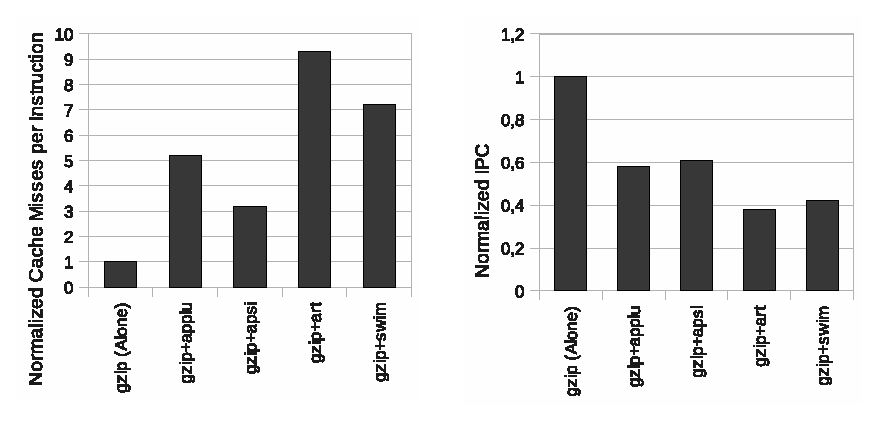
\includegraphics[width=\widefigure]{images/chandra_gzip}
\caption{\figurecaption{gzip miss rate}}
\label{fig:gzip_miss}
\end{figure}

The picture shows gzip's number of cache misses per instruction and instruction per cycle (IPC), when it runs alone compared to when it is
co-scheduled with different threads, such as applu, apsi, art, and swim. All the bars are normalized to the case where gzip is running alone.
It is interesting to note how gzip's number of cache misses per instruction increases significantly compared to when it runs alone. Infact, it increases 
by 3x when it runs with apsi and by 9.5x when it runs with art, 7.3x when it runs with swim.
Consequently, the IPC is affected differently. It is reduced by 35$\%$ when gzip runs with apsi, but reduced by 63$\%$ when gzip runs with art. 
Although not shown in the figure, art, apsi, applu, and swim's cache miss per instruction increases less than 15$\%$ when each of them runs with gzip. 

In terms of fairness, gzip's significant slow down can easily result in \textbf{priority inversion}. 
For example, if gzip has a higher priority than art, for gzip to achieve a higher progress rate, it has to be assigned more than three times the 
number of time slices compared to that assigned to art. Otherwise, to the end users, gzip may appear to be starved. In terms of throughput,
gzip's significant slow down reduces the overall throughput because the utilization of the processor where gzip runs on is also significantly reduced. 
Furthermore, it is possible that the co-scheduled threads's working sets severely overflow the cache and create a \textit{trashing} condition.

In briefly, there are at least three problems that may happen and render the OS schedule ineffective.
The first problem is \textit{thread starvation}, which happens when one thread fails in competing for sufficient cache space necessary to make 
satisfactory forward progress. The second problem is \textit{priority inversion}, where a higher priority thread achieves a slower forward
progress than a lower priority thread, despite the attempt by the OS to provide more timeslices to the higher priority thread.
This happens when the higher priority thread loses to the lower priority thread (or other threads) in competing for cache space. 
To make things worse, the operating system is not aware of this problem, and hence cannot correct this situation (by assigning more timeslices to the 
higher priority thread). The third problem is that the forward progress rate of a thread is \textit{highly dependent} on the thread mix in a co-schedule. 
This makes the forward progress rate difficult to characterize or predict, making the system behavior unpredictable. Unfortunately, despite these problems, 
cache implementations today are thread-blind, producing unfair cache sharing in many cases.

As I said in the first chapter, in theese years were developed some ideas about how to make a scheduler cache-aware.
This chapter aims to show the general structure and strategies used to model cache behaviour followed by theese algortihms, that are the most interesting 
part of theese type of heuristics.

%%%%%%%%%%%%%%%%%%%%%%%%%%%%%%%%%%%%%%%%%%%%%%%%%%%%%%%%%%%%%%%%%%%%%%%%%%%%%
\section{Survey on cache architecture}
\label{sec:s1}

Over the years, cache architectures have always played an important role in system performance. Hundreds of research papers show how performance
can be improved using multi-level caches on a single-processor machine. Multicore systems introduce new challanges for cache designer, because cache memory 
is a shared resource, therefore issues related to how a core access to cached data and how the coherence regarding the access from different processors 
to the same cached data is guaranted are unavoidable. Furthermore, caches play an important role in managment of comunication betwen different core.
This section aims to show which are most important factors introduced in cache architecture to take in consideration during the development of cache aware
alogrithms from scratch. Theese cache characteristics are common in both general purpose and embedded systems.

%-----------------------------------------------------------------------------
\subsection{Cache coherent protocols}

Usually in multicore architecture, there is a private L1 cache for each core, and there is a L2 or L3 cache shared among all cores (SMP), or among cores 
that belong to the same node (NUMA). Shared cache is one of the most critical resources in multicores.

As for all types of shared resources, also for shared cache it's necessary to ensure integrity of the shared data.
Before to analyze mechanisms used to ensure data integrity, it is necessary pay attention to the difference between two terms: consistence and coherence.
When two or more CPUs operate on a shared variable and one of these CPUs modify the variable, it is necessary that the information regarding
this change of value be communicated to the other CPUs. Consistence refers to 'when' this change in memory data is available to other CPU cores.
Coherence refers to 'how' the change is communicated between the processors. Therefore, to ensure correctness of cache operations, it is necessary define
when a modified value must be made visible to another processor's read instruction, this is the consistency model, and define the rules used to comunicate 
memory update between different cores, this is coherence protocol. In briefly a cache coherence protocol is the mean used to maintains consistency between
all the cache in the system. Existing coherence protocols are classified based on the mechanism by which they ensure cache coherence: 

\begin{itemize}

\item Snooping based protocols: Each cache monitors address lines of shared bus for every memory transaction made by remote processors. Appropriate action
is undertaken when data locally cached is modified by this transaction, for example: a write by a remote processor into a data address locally cached 
results in an invalidation of the local cache copy .

\item Snarfing based protocols: A cache controller watches both address and data in an attempt to update its own copy of a memory location when a second 
master modifies a location in main memory. When a write operation is observed to a location that a cache has a copy of, the cache controller updates its 
own copy of the snarfed memory location with the new data.

\item Directory-based protocols: Shared data are placed in a common directory that maintains the coherence between caches processor caches. 
This directory acts as a look-up table for every processor to verify coherence and consistency of data that is currently being read or updated.

\end{itemize}


The first two mechanisms are typical of the SMP architecture, while the last is used in large point-to-point inter-processor communication network 
architectures. Snooping protocols became popular and widely accepted with multiprocessors systems since it required minimal change to the pre-existing 
physical shared bus interface to the memory. The inherent broadcasting property of the snoop protocols makes it simple to implement but places an upper 
limit on scalability.
Over the years, several snooping based cache coherence protocols were developed. The most common is MESI protocol.
With this protocol, every cache line is marked with one of the following states:

\begin{itemize}

\item Modified
The cache line is present only in one of the local caches, and it has been modified from the value in main memory. Write on a modified cache line are 
allowed, reads are a bit complicated. The local cache that owns a modified cache line must intercept (snoop) all attempted reads (from all of the other 
caches in the system) at main memory location that correspond to modified cache line, forcing them to back off, then writing data to main memory and change
state of cache line to shared state.
 
\item Exclusive
The cache line is present only in the current cache, and it matches main memory. It is possible read/write lines in this state. A cache that own
line in exclusive state must snoop all read transaction from all other cache and if it intercepts some read that regard owned cache line, it changes
state of that line from exclusive to shared.

\item Shared
Indicates that this cache line may be stored in other caches and it matches the main memory. It is possible read cache line in this state. Writes to a shared
cache line are allowed but before to perform the operation, it is necessary invalidate all other copies in other caches.
A cache that holds a line in the Shared state must listen for invalidation from other caches, and discard the line (by moving it into Invalid state) on a 
match.

\item Invalid
Indicates that this cache line is invalid, read/write operation on invalid cache line are denied

\end{itemize}

Cache coherence protocols play an important role to improve efficiency of the read/write in cache. There are a lot of variant of MESI protocol, the most 
recent variants are MESIF and MOESI.

The former protocol adds Forward state. It is only relevant for the L3 cache. This state indicates that only one cache should act as a designated responder 
for any requests for the given line. With the standard MESI protocol, a request for cache line will receive a response from each cache that contains that 
line in the shared state. Instead, with MESIF protocol a request will be responded to only by the cache holding the line in the Forward state.
A cache line shared among multiple processors will be in forward state in only one L3 cache. This protocol is used in new Intel microarchitecture Nehalem 
and it is designed for ccNUMA. The aim of this new state is to reduce communications between cache.

The latter protocol add Owned state. A cache line in this state holds the most recent, correct copy of the data. Only one processor can hold the data 
in the Owned state, all other processors that contains a copy of that data must hold the them in the shared state. A copy of data in main memory can be 
incorrect. A cache line in owned state may be changed to the Modified state after invalidating all shared copies, or changed to the Shared state by 
writing the modifications back to main memory, furthermore cache lines must respond to a snoop request with data. 
It is clear that the aim of this protocol is to avoid the need to write a dirty cache line back to main memory when another processor tries to read it. 
With the Owned state, processor can supply the modified data directly to the other processor. This is beneficial when the communication latency and 
bandwidth between two CPUs is significantly better than to main memory. An example of MOESI implementation is present in AMD Shanghai microprocessor.

%-----------------------------------------------------------------------------
\subsection{Inclusive and exclusive cache}

Another important architecture detail that affect performance is if a cache is inclusive or exclusive.
An inclusive cache means that all data available in higher level cache are contained also in the last level cache, namely in shared cache.
An exclusive cache means that data is present only in one cache.

It is clear that theese two architectural policy are focused on two different aspects. The first policy greatly reduces snoop traffic because if a core 
doesn't find requested data in any of its cache level, it knows the data it is also not present in any other core's cache. The second policy, instead, 
allows to store more data than an inclusice cache, because for each data only one copy is stored.

An example of inclusive L3 shared cache is implemented in Intel Nehalem microarchitecture. In this implementation to insure coherency across 
all caches, the L3 cache line has additional flags that keep track of which core the data came from and a core valid bit that indicate that cache line 
is present in some core's cache. If the data is modified in L3 cache, then the L3 cache "knows" if the data came from a different core than last time 
and that the data in the first core needs its L1/L2 values updated with the new data. This greatly reduces the amount of traditional "snooping"
coherency traffic between cores. Moreover the core valid bit doesn't ensure that a L3 cache line is placed also in an higher level cache, because unmodified
cache lines may be evicted from a core's cache without notification of the L3 cache.

An implementation of exclusive cache can be found in AMD's Shanghai processors. Theese cpus present an interesting implementation of this type of cache
architecture, because L1 and L2 are exclusive cache, but last level shared cache (L3) is a not-inclusive cache.
Not-inclusive architecture is a variant of exclusive architecture, becasue if a cache line is transferred from the L3 cache into the L1 of any core, the 
line can be removed from the L3. According to AMD this happens if it is "likely" that the line is only used by one core, otherwise a copy can be kept in 
the L3. About how the cpu can "understand" if a line will be used only by one core, AMD has not revealed details. Nowadays, an inclusive cache is 
preferred over an exclusive cache, because it simplifies the problem of cache coherence. 

\begin{figure}[htbp]
\centering
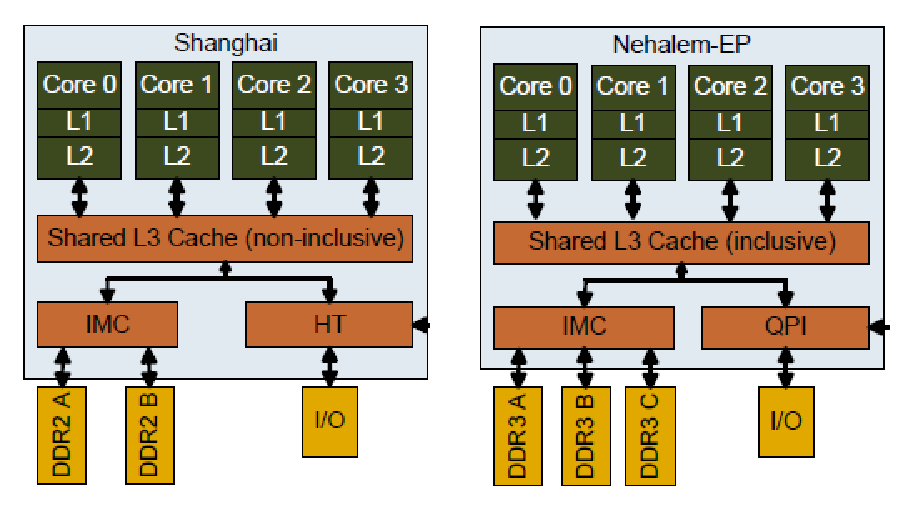
\includegraphics[width=\widefigure]{images/neh_amd.eps}
\caption{\figurecaption{AMD Shanghai and Intel Nehalem}}
\label{fig:neh_amd}
\end{figure}

To get a sense of how cache coherence and an inclusive or exclusive of cache impact on system performance, it is possible to look over the work made by 
Molka et al. \cite{molka}. They have compared perfomance of MESIF protocol applied to inclusive cache (Intel Xeon 55** Nehalem) and MOESI protocol applied 
to an exclusive cache (AMD Shanghai), see figure \ref{fig:neh_amd}. Theese processors tested are multithreaded and ccNUMA dual-socket SMP systems. 
In the table \ref{fig:tab_lat} are showed read latencies recorded during test.

\begin{figure}[htbp]
\centering
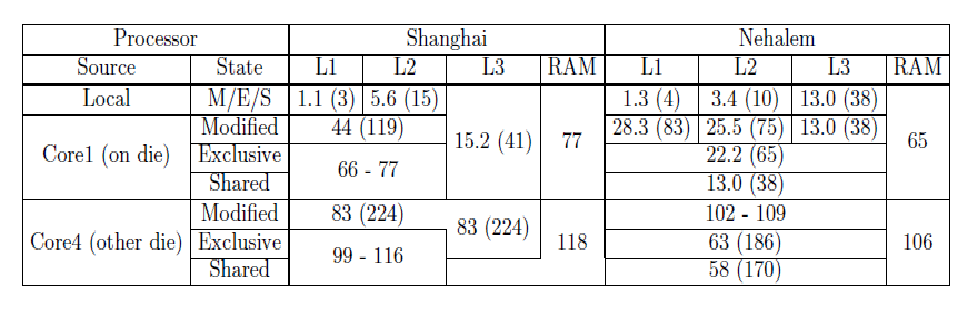
\includegraphics[width=\widefigure]{images/tab_lat.eps}
\caption{\figurecaption{read latencies}}
\label{fig:tab_lat}
\end{figure}

\begin{description} % off - on chip

\item[on-chip latencies] Theese data measure access time to the cache of other cores on the same die. We will see that to have an inclusive cache or not
influence strongly this type of latencies. 

\textbf{Nehalem:} A \textit{Shared} cache line in L3 is guaranted to be valid and it could be in shared or forward state, it can be accessed within 13 ns. 
An \textit{Exclusive} cache line that has core valid bit set in L3, may has been modified in higher level cache, this fact forces the L3 cache to check the 
coherency state in the core, therefore the latency increase up to 22.2 ns, furthermore, in the this type of cache, exclusive cache lines can be silently 
evicted from higher level cache and remain only in L3. The check on coherency state is made also for theese lines that are only in L3 cache.
A read of \textit{Modified} cache line present in other on-chip L1/L2 requires 25.5/28.3 ns, but if a modified line is evicted from L1/L2, it is required a 
write-back in L3 and an update of the core valid bits. It means that future access at that line will has a latency of 13 ns again.

\textbf{Shanghai:} A \textit{Shared or Exclusive} cache lines from higher level caches need to be fetched from the cores or main memory if no copy exists 
in the non-inclusive L3 cache. Latency showed in the table indicate that request for lines in theese state are serviced by main memory.
A \textit{Modified} state it's the only state that allow to avoid access to main memory.

\item[off-chip latencies] Theese data measure access time to the cache of other cores on another die. Theese latencies include additional penalty for the
QPI/HT data transfer. We will see that cache coherence protocol influence this type of latencies.

\textbf{Nehalem:} Thanks to inclusive cache, the access to unmodified data is fast. Latency for \textit{Exclusive} cache line include a snoop of one core 
(63 ns), \textit{Shared} cache line don't require snoop (58 ns). Moreover, latency for \textit{Modified} lines is higher (> 100 ns), becasue the MESIF 
protocol requires a write back to the main memory.

\textbf{Shanghai:} Cache lines in \textit{Shared} state are fetched from main memory (> 99 ns), L3 can satisfies request for \textit{Exclusive} cache lines 
(83 ns). Cache line in \textit{Modified} state can be forwarded to the requesting core from all cache levels, furthermore, thanks to MOESI protocol, a 
modified cache line in the remote cache can switch to the Owned state and avoid to be written back to main memory.

\end{description} % end on - off chip

It is intersting to note how  accesses to remote caches on Shanghai are slower than accesses to the local RAM (83 vs. 77 ns). 

%-----------------------------------------------------------------------------
\subsection{Cache Hardware prefetcher}

Finally, it is necessary to spend a few words about prefetching. Prefetcher is an hardware component that tries to predict which memory addresses are
going to be used by the program, in order to load needed data in cache memory just in time.
Typical technical workloads often access memory in regular and sequential patterns, therefore, with a smart prediction mechanism, a prefetcher can select 
and load right data and, in this way, reduce memory latency. The key point to build a good prefetcher is to design prediction mechanism.
In literature there are many ideas to solve this problem. An example of concrete solution is the Intel Smart Memory access. This system was introduced
with Intel Core microarchitecture. In this system there are two prefetchers to the Level 1 data cache and the traditional prefetcher to the Level 1 
instruction cache. In addition there are two prefetchers associated with the Level 2 cache and shared between the cores. In total, there are eight
prefetchers per dual-core processor. 
In order to improve the accuracy of the prediction, the prefetcher system tags the history of each load using the Instruction Pointer (IP) of the load. 
For each load, the prefetcher builds a history and keeps it in a suitable history array. Based on load history, the prefetcher tries to predict the 
address of next load accordingly to a constant stride calculation (a fixed distance or "stride" between subsequent accesses to the same memory area). 
At this point, the prefetcher generates a prefetch request with the predicted address and brings the resulting data to the Level 1 data cache.
In literature, this kind of prefetchers are called \textit{strided} prefetcher.
Other architectures, such as Power ISA\_2.06, that use a strided prefetcher, introduces cache instructions to hint prefetch system for data prefetching.
With this instructions an application can specify direction, depth, no of units and so on. In this way, the programmer has a low level control on 
data prefetched.

Another category of prefetcher are \textit{non-strided} data prefetcher. They are very useful for accessing complex and irregular data structures as 
linked list, B-Trees etc. There are different techniques to implement theese prefetcher, one of theese is "pattern history based prefetcher". 
In this approach, the prefetcher tracks the addresses of misses and tries to identify specific patterns of misses that occur together (temporally). 
Once a pattern of misses has been detected, the prefetcher will find the first miss in the pattern. When this first miss occurs again, the prefetcher 
will immediately prefetch the rest of the pattern. For traversing a complex data structure like a linked list, this would be a fairly effective approach.
Recently AMD has announced that it will employs a non-strided prefetcher in its brand new Bulldozer microarchitecture, but it has not revealed details on 
implementations.

%%%%%%%%%%%%%%%%%%%%%%%%%%%%%%%%%%%%%%%%%%%%%%%%%%%%%%%%%%%%%%%%%%
\section{Classification of cache-aware Scheduling algortihms}

Cache aware scheduling policies can be classified according to type of strategy followed. They are divided in \textit{data locality} and 
\textit{temporal locality} policies. The former type is focused on a smart allocation of resources in cache. Theese policies partition cache memory in order
to every task may use a dedicated area in cache memory and then, reduce inter-thread cache interference and miss rate.
The latter type is focused on cache reusability. Theese policies schedule tasks that subsequently will access at the same data, reducing miss rate.

%-----------------------------------------------------------------------------
\subsection{data locality policies} 

Theese policies are focused on the use of Last Level shared Cache (LLC) made by scheduled tasks. They can be used both for Real-time and Fair tasks. 
They don't take care about core-local cache (usually L1) or other shared resources like interconnects. In literature, data locality is the most developed 
type of cache aware policies, because they can be integrated in every OS and are relatively simple policies to develop. Now I will show two examples of 
data locality policies and how they are implemented.

\begin{description}
\item[Cache aware Fixed priority policy:] To understand this type of policy assume this situation: consider a multicore platform consisting of $M$ cores 
with an on-chip LLC, and a task set $\tau$, in which each task $T$ releases a job $J_i$ every period $p(T)$. Every released job is characterized by a 
worst-case execution time (WCET) denoted by $e(T)$. It means that each job released by task $T$ has a maximum duration of $e(T)$. For each job is defined 
the number $A(J_k)$ that represents the total cache space size used by it: we define this space as per-job \textit{working set sizes} (WSS). 
For simiplicity we assume that each job generated by a task $T$ use the same number of partition, therefore it is possbile to express $A(J_k)$ as $A(T)$. 
The quantity $e(T)/p(T)$ is called the utilization of $T$, denoted $u(T)$. The deadline $d(J_k)$ of a job $J_k$ coincides with the release time of job 
$J_{k+1}$. If job $J_k$ completes its execution after time $d(J_k)$, then it is \textbf{tardy}. For some scheduling algorithms, tardiness may be bounded 
by some amount $B$, meaning that any job $J_k$ will complete execution no later than time $d(J_k)+B$. Finally, assume that tasks have fixed priority.
This model describe very well a typical Real-time application.

A job $J_k$ is scheduled for execution if:

\begin{enumerate}
	\item $J_k$ is the job of highest priority among all waiting jobs,
	\item There is at least one core idle
	\item There is enough cache space, i.e. at least $A(J_k)$ , is available.
\end{enumerate}

\begin{table}[htbp]
\begin{center}
\begin{tabular}{l|c|c|c}
	\hline
	& $p(T)$ & $C(T)$ & $A(T)$ \\ \hline
	$T_1$ & 3 & 2 & 1 \\ \hline
	$T_2$ & 4 & 3 & 2 \\ \hline
	$T_3$ & 5 & 3 & 2 \\ \hline
	$T_4$ & 8 & 3 & 1 \\ 
	\hline
\end{tabular}
\caption{An example task set}
\label{tab:cache_task_set}
\end{center}
\end{table}

\begin{figure}[htbp]
\centering
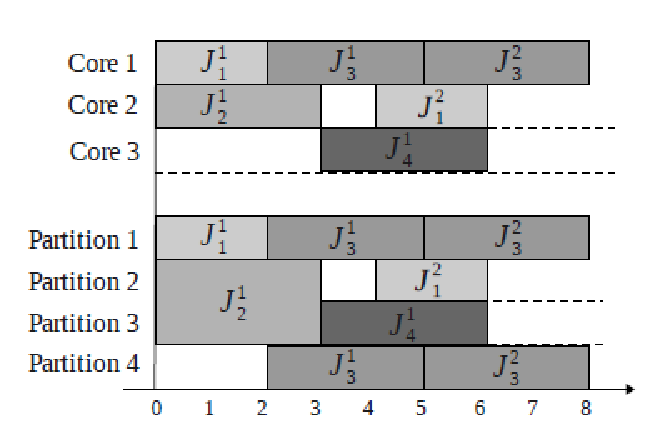
\includegraphics[width=\widefigure]{images/schedule.eps}
\caption{\figurecaption{Example of scheduling performed by cache aware policy}}
\label{fig:sched_example}
\end{figure}

Figure \ref{fig:sched_example} shows how the task set in Table \ref{tab:cache_task_set} is scheduled by the policy. The index of each task 
indentify the task and indicate the priority of the latter. Higher priority is 1 and lower priority is 4. In the picture jobs are represented in this way: 
$J_{\alpha}^\beta$, where $\alpha$ represents which task has released the job, and then also its priority, and $\beta$ is an index that identify the job.
We assume that co-scheduled jobs use not-overlapped cache partitions.

At time 0 all jobs are released. At this time, the job $J_{4}^1$ can not be executed because it has lower priority than $J_{3}^1$ and the latter can not be
scheduled since there is not enough idle cache partitions available.

It is clear that the aim of the described policy is to avoid cache trashing that occurs when the amount of space required by co-scheduled jobs is greater 
than the dimension of LLC. A very important assumption made in this policy to achieve this goal is that all jobs use not-overlapped 
partition of cache. This fact simplifies the scheduling problem, because it's enough make a check on amount of cache space occupied by co-scheduled jobs to 
infer if cache thrasing occurs. Moreover, in practice cases, it is not always true, because it greatly depends on type of application executed.


\textit{\textbf{Mechanisms and examples}} They key mechanism to reach this goal is profiler that we will call \textit{co-scheduler}. At runtime, the 
co-scheduler tries to infer what is the WSS of each scheduled task and provide theese informations to scheduler. The challenge is how to do this job. 
Calandrino et. al \cite{calandro} propose an interesting implementation of co-scheduler and of this type of policy.

The implementation is focused on Soft Real-time tasks, its solution is quite simple: it makes EDF cache-aware. Standard EDF algorithm gives higher priority 
to the task with earlier deadline in order to schedule it as soon as possibile. A cache-aware EDF is very similar to classic EDF: it "promotes", that is 
increase priority, of the job with the smallest WSS, in this way jobs on a runqueue are ordered by WSS.

The algortihm uses two separate run queues for eligible jobs: the former is EDF-ordered, the latter is a "promotion" queue. In this queue, jobs are ordered
from smallest to largest WSS. The job in front of this queue is "promoted", that is its priority was increased and, for this reason, it remains at the front
of the queue and it will be the next task to execute. But if there are tardy jobs, the algorithm schedules the job at the head of the EDF-ordered queue.
When the heuristic picks a task from promotion queue, it checks if it will cause cache thrashing. For this reason, the scheduler mantains a variable with 
the total amount of the WSSs allocated, that is the cache space allocated. If this value plus the WSS of the job to schedule exceeds the cache space size, 
thrashing will occurs. In this case, the core remains idle and the job waits for some job that frees cache resources.
Obiouvsly task priorities are respected, it means that a task with the smallest WSS is promoted only if it has the higer priority.

\begin{figure}[htbp]
\centering
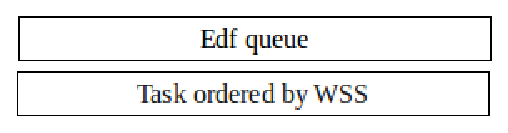
\includegraphics[width=\widefigure]{images/edf_wss.eps}
\caption{\figurecaption{queues used in the algorithm}}
\label{fig:edf_wss}
\end{figure}

To compute the WSS used by each task, the co-scheduler divides the total cache misses observed over all profiled jobs by the total number of profiled jobs, 
and multiplying the result by the cache line size. All the profiled jobs belong to the same task. The co-scheduler discards measures obtained by jobs that 
cause cache thrashing. Cache misses are recorded using performance counters. At the beginning of an application, there is not any measure about cache miss, 
therefore the co-scheduler requires a bootstrapping phase in order to get necessary measures. This phase converge pretty fast to a reasonable result.

It is interesting to note, that in this implementation the only mean to avoid cache trashing is a check on amount of WSSs used by scheduled tasks.
This is a sub-optimal solution because cache trashing can occurs also in those cases where the total amount of WSSs is less than total amount of cache
space. The reason is simple: the WSSs of two jobs could be overlapped, furthermore, also under hypotesis of non-overlapped WSSs, check on WSS is sufficient
to prevent cache thrashing only if the cache is fully associative, because every line in main memory can be mapped on any cache line but, in a N-way 
set associative cache, a line in main memory can be mapped only within a certain set. For this reason, if a task occupies cache line used by a co-scheduled 
task, cache trashing will occcurs. Calandrino et al. test their algorithm with Soft Real-Time multimedia application and, according to results showed 
\cite{calandro}, it seems that this sub-optimal solution is quite effective, at least with this kind of applications.

\textbf{\textit{Advantages and drawbacks}} This policy presents a clear drawback: it may waste resources. According to rules previously showed, if there 
is an idle core, but not enough cache space, a task may not be scheduled and, in this way, degrade throughput. Moreover, the policy improves predictability 
of the application, and this aspect make this policy very indicate for Real-time system, where predictability is a very important aspect.

There is another important advantage related to improvement of predictability. On single-core systems there are well-developed techniques for timing 
analysis of embedded software. Using these techniques, the WCET of real-time tasks may be estimated, and then used for schedulability analysis. 
In multicore systems theese tecniques can't be used, because, as we have seen, cache behaviour (hit or miss) is unpredictable because it depends on which 
tasks are co-scheduled, therefore WCET can be variable and very difficult to estimate. With the analyzed policy, it is possible perform a proper cache 
isolation, that make cache behaviour more predictable and then it becomes feasible to execute a system-level schedulability analysis using existing WCET 
analysis techniques. For details on WCET analysis for Real-time system in multicore platform see \cite{guann}


\item[Fair cache sharing policy:]

This policy is focused on Fair tasks, therefore it considers an application model with less constraints than to that considered by
Calandrino et al. This implementation ensures \textit{fair cache sharing}, that is a more strength strategy than to only avoid cache trashing.

As we have previously seen, a bad combination of coscheduled tasks may cause cache thrashing and, consequently, a variation on task's instruction per cycle
(IPC) that determines task's performance variation. But, if co-scheduled tasks sharing cache in a fair way, they can allocate needed resources in cache and
they experience the fair IPC, that is the IPC that ensure the best overall performance. The mechanism used to ensure the fair IPC is to modify CPU timeslice 
assigned to a task, in this way, each task always run as quickly as it would under fair cache allocation, regardless of how the cache is actually allocated.

\begin{figure}[htbp]
\centering
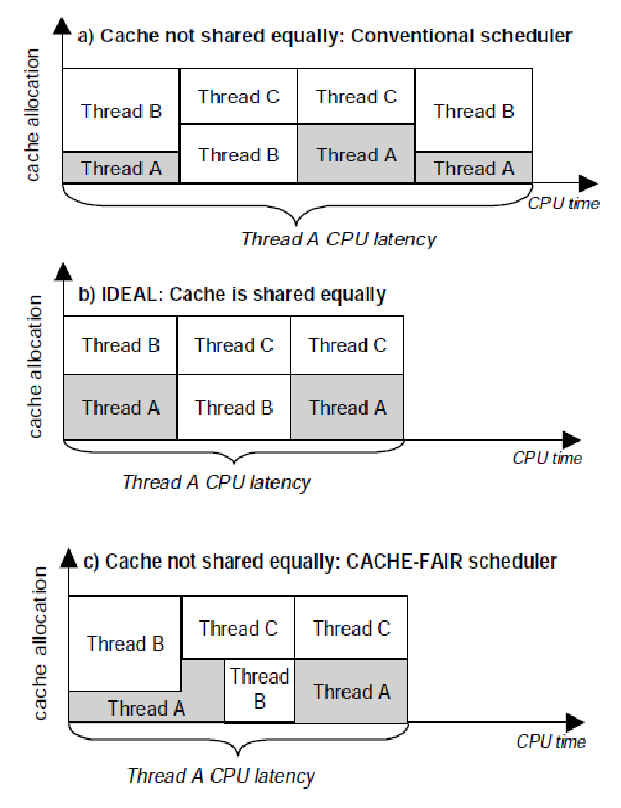
\includegraphics[width=\widefigure]{images/fed_cases.eps}
\caption{\figurecaption{queue used in the algorithm}}
\label{fig:fed_cases}
\end{figure}


In figure \ref{fig:fed_cases} is represented what the alorithm tries to do. Each box corresponds to a task. The height of the box indicates the amount of
cache allocated to the thread. The width of the box indicates the thread's CPU timeslice. The area of the box is proportional to the amount of work 
completed by the thread. Stacked thread boxes indicate corunners. In situation (a) is represented the ideal case, where all tasks share equally 
cache. In the case (b) is represented a real case where tasks don't share equally cache and, for this reason, Task A needs more CPU time to execute
all its job. Case (c) represents how is possible to ensure fair cache sharing: Task A can't make forward progress, so CPU timeslice of task A is increased 
and, at the same time it decreases timeslice of task B to mantain balanced CPU sharing. This is what the algorithm does. 


\textit{Mechanism and examples:} An implementation of this policy is developed by Fedorova et al. \cite{fedorova}. The algorithm is divided in two phases: 
sampling and scheduling. During the sampling phase, the co-scheduler gathers performance data and uses it to estimate the task's fair miss rate. During the 
scheduling phase, the scheduler periodically monitors the task's performance and adjusts the task's CPU timeslice if its actual performance deviates from 
its fair performance.

The fair miss rate and fair IPC of a task are estimated via performance counters, executing this experiment: different groups of corunners are formed, 
the task which we want to estimate fair miss rate is executed togheter to each group. At the end of execution, miss rates of each executed task are 
recored. Theese measures correspond to one data sample. It is necessary to collect at least ten data sample for each task, in order that each task has 
completed at least 100 million of instructions, to eliminate effects of compulsory misses. At the end of the sampling phase, the co-scheduler estimates the 
fair miss rate using a linear regression analysis and, according theese informations, also fair IPC is computed. In the scheduling phase, the scheduler 
monitors the task's IPC, again via performance counters. According to the difference between IPC measured and task's fair IPC, the scheduler adjusts task's 
CPU timeslice.

\begin{figure}[htbp]
\centering
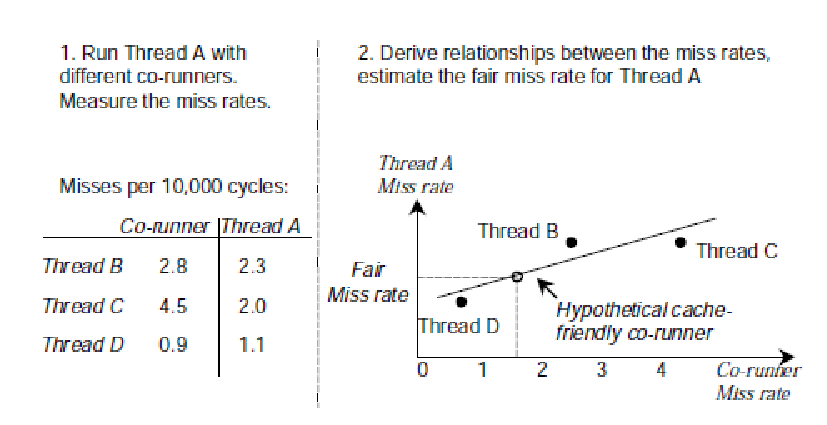
\includegraphics[width=\widefigure]{images/fedorova.eps}
\caption{\figurecaption{step of co-scheduler}}
\label{fig:fedorova}
\end{figure}


In Figure \ref{fig:fedorova} is reassumed how fair miss rate is estimated. Fedorova et al. found that that a linear function is the best approximation of 
relationship between co-runnners miss rates.

The overhead of sampling phase is fixed and it is repeated every time a thread has completed one billion instructions, while the check on a task's IPC
is made every 50 million instrucitons executed. When to check task's IPC and when to perform sampling phase is decided according to empirical observations
made by the developers of the algorithms.

It's important to note that this algorithm does not esablish a new CPU sharing policy but simply enforce existing policies. For example, if the 
system is using a fair-share policy, the cache-fair algorithm will make the cache-fair threads run as quickly as they would if the cache were shared 
equally, given the number of CPU cycles they are entitled to under the fair-share policy. Furthermore, the algorithm doesn't add any additional data 
strcuture, but simply requires only to record fair miss rate and fair IPC for each task.

\textbf{\textit{Advantages and drawbacks}}
Unlike previous example, this algorithm don't waste resource, moreover it use a more complex co-scheduler than that implemented by Calandrino et al, 
because it has to estimate fair miss rate of each task. According some statistical considerations, two corunner task experience fair cache sharing, if 
their miss rate is similar and that miss rate is the fair miss rate. To determine this value for each task, a possible approach consist of executing a task 
with all available corunner, but this approach is not feasible. The solution adopted by the co-scheduler, instead, consist of to run each task with a small 
number of possible corunner and use miss rates measured to derive a relationship between the miss rates of the task analyzed and its co-runners, and use 
that relationship to estimate task's fair miss rate. This procedure could introduce an higher unpredictability in the application and for this reason, that 
this algorithm couldn't be suitable for Real-Time systems, where predictability is required.

\end{description}

%-----------------------------------------------------------------------------
\subsection{temporal locality policies} 

The idea behind this type of policies is very simple, but in practice it is more complex than the idea behind data locality policies. Theese policies 
require complex infrastructure and nowadays only few research works has developed polcies of this type. An interesting implementation of this type of policy
can be found in COOL project \cite{COOL}. Recently Yang et al. \cite{taiwan} has implemented a scheduling algorithm inspired to theese policies and 
naturally the concept of taskaffinity is a simplify implementation of temporal locality policies.

\begin{description}
\item[cache reusability policy]
The key point to maximize reusability of data in private cache is data sharing among tasks. If two threads, or in general two task, sharing common data, 
they are scheduled subsequently on the same cpu, in this way, it's more likely to reuse the same data in private cache.
According this observation, tasks are partitioned in groups called \textit{sharing groups}. Tasks that share the same resources are put in the 
same sharing group. After partitioning, the scheduler assigns the same cpu at all tasks that are in the same sharing group, in this way they will use 
always the same private cache. 

Instead, to maximize reusability of data in shared cache it is necessary to improve the opportunities that the subsequently scheduled tasks could reuse the 
data accessed by the current tasks at the scheduling point.

\begin{figure}[htbp]
\centering
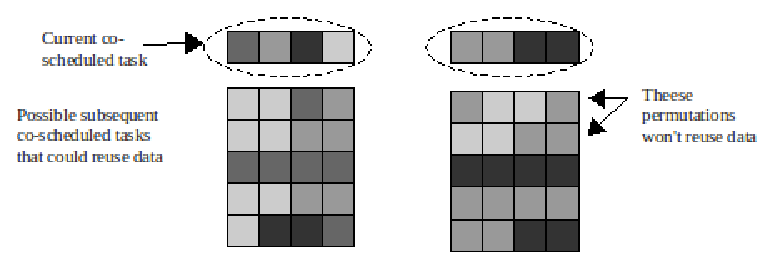
\includegraphics[width=\widefigure]{images/cosched_permutation.eps}
\caption{\figurecaption{task permutation}}
\label{fig:cosched_permutation}
\end{figure}

In figure \ref{fig:cosched_permutation} are represented possible permutations of co-scheduled tasks that can reuse content in shared cache. 
Each square represents the data set used by a scheduled task, squares with different colours represent different data set. In the case (a), four tasks are 
co-scheduled and they access to four different data sets, in the case (b) four co-scheduled tasks access to only two different data sets. To reuse the 
data in the cache, it is necessary schedule tasks that use data sets that have been accessed by current co-scheduled tasks subsequently. Therefore, more 
data sets are accessed by current co-scheduled tasks and there will be more opportunities that the subsequent coscheduled tasks could reuse the data in the
shared cache. For example: in situation (a) there are $4^4$ permutations of co-scheduled tasks that could reuse the data, but only $2^4$ in situation (b). 
According this observation, the scheduler should schedule the tasks using as many data sets as possible, but at one important condition: the total amount 
of data set used by co-scheduled task, must be less than the total cache space, in order to avoid cache trashing.

The interesting thing, is that the two described maximization goals are not in conflict each other. The explanation is straightforward: each core executes 
a task that belongs to different sharing group, therefore co-scheduled tasks would access \textbf{different data sets}, in this way, the number of data sets 
accessed in shared cache is maximazed.

According to this theory, it is possible to list the rules applied this kind of policy:

\begin{itemize}
	\item Co-schedule tasks that belong to different sharing groups. 
	\item Schedule a task only if it doesn't cause cache thrashing.
\end{itemize}

\textit{\textbf{Mechanism and examples:}} An implementation of this policy is developed by Yang et al. \cite{taiwan}. Before describing mechanism used, it is
necessary to remember that each task belongs to one sharing group denoted with $SG_i$ and it is characterized by its working set denoted with $TW_i$.
Before to start, the algorithm assigns each sharing group to one cpu: if number of core (NC) is less than number of sharing groups (NS), a cpu will execute 
more than one sharing groups, see fig. \ref{fig:possible_cosched}.

\begin{figure}[htbp]
\centering
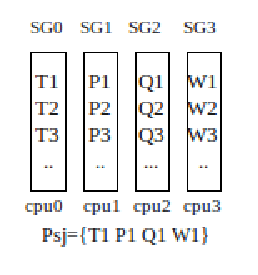
\includegraphics[width=\widefigure]{images/possible_cosched.eps}
\caption{\figurecaption{possible coschedule for a task j, in this case task A}}
\label{fig:possible_cosched}
\end{figure}

The heuristic is divided in two phases. In the first step, the algortihm chooses a task from each sharing group for a total of NC tasks, in this way, it
has defined a possible co-schedule ($PS_j$). It computes the sum of working set size (SWSS) of the $PS_j$ selected, if SWSS is greater than dimension of 
shared cache, $PS_j$ is discarded. This procedure is repeated for all possible $PS_j$. At the end, all filtered $PS_j$ that fit into the shared cache are 
put in a queue called $C$ and waiting for the next phase.

Define the \textit{sharing number ($SC_j$)} as the number of different sharing groups belong to a possible filtered co-schedule $PS_j$. In the 
next step, elements present in queue $C$ are orderd according their $SC_j$. In order to schedule tasks that access the most different data sets, the 
algorithm select tasks that belong to $PS_j$ with the maximum $SC_j$.

If $C$ is empty, it means that there isn't any possible co-schedule $PS_j$ with the total working set size $TW_j$ that fit in shared cache. Also in this 
case, the algorithm would aim to minimize the shared cache misses by choosing the possible co-schedule with the maximum $SC_j$ and with smallest $TW_j$.

An interesting aspect of this implementation, is that it is possbile to reduce also cache coherence overhead, the reason is very simple. Tasks that belong 
to two different sharing groups don't share data, otherwise they should be in the same groups. It means that lines used in private cache by
a co-scheduled tasks that are in different groups, won't never be in shared, but only in modfied or exlusive state. in this way, the overhead due to 
management of cache coherent shared state is reduced. 

Yang et al. implemented their algorithm in the scheduler present in Threading Building Blocks (TBB) that is a multrithreading library developed by Intel. 
This library allows to programmer to specify which is the working set of each threads and this information is just what it needs to implement their policy. 


\textbf{\textit{Advantages and drawbacks}}
This policy is an improvement of data locality policies, because, also in this case, it is essential to prevent cache trashing in LLC,
exploiting the same mechanisms used in data locality policies.

An important aspect of this policy is that it deals with cache coherence, that, as we have seen in previous section, is a very important factor that 
influence system performance. A drawback, is that to implement this policy is required an infrastructure that provide the same informations used in 
data locality policies, that is how much cache space a task use, and in addition, which are addresses used by task, that is a very difficult information
to obtain. To resolve this problem, the algorithm involves the programmer providing him a suitable API to influence the scheduling choices. This fact 
means to modify appllication code with additional functions. 
\end{description}





\cleardoublepage
\chapter{Improving TaskAffinity}
\label{cha:Improve taskaffinity}

In this chapter, we analize the behaviors of the current task-affinity
implementation considering different architectures and benchmarks.  This
analysis is two fold: on one side it allows to understand why the current
task-affinity implementation is not effective on some architectures, e.g. the
Intel Xeon, on the other which are the points of task-affinity logic that can be
optimized in order to improve an application \emph{throughput and
predictability}.

%%%%%%%%%%%%%%%%%%%%%%%%%%%%%%%%%%%%%%%%%%%%%%%%%%%%%%%%%%%%%%%%%%%%%%%%%%%%%
\section{Scheduler architecture on 2.6.34}

Now I will briefly introduce which are the parts of the scheduling procedure 
interested by the task-affinity logic and which are the most important changes 
carried out from 2.6.31 kernel version to 2.6.34.

%-----------------------------------------------------------------------------
\subsection{Task wake up management}

The scheduling procedure for a task starts when it wakes up. A task can wake up
for different reasons, i.e. a semaphore becomes unlocked or a new task creation.  In all those cases different
kernel functions are called, but at the end they call the \texttt{try\_to\_wake\_up} function:

\lstset{basicstyle=\footnotesize, language=c, captionpos=b, frame=single, label=lis:APIttwu}
\lstinputlisting{API_ttwu.c}

where $p$ is the to be waken task.
This function follows these steps:

\begin{enumerate}
\item Disables kernel preemption, locks the runqueue where $p$ was last executed and check 
if $p$ is not already waken up and it is not already on a runqueue. In the first case the 
function releases lock and exits, in the second case the function check if a
\textit{push} is necessary. Further details about these if statements will be
describe thereafter. If the two checks fail, $p$'s state is changed in the TASK\_WAKING, the
lock on runqueue is released and \texttt{select\_task\_rq}, a wrapper for a 
class-specific \texttt{select\_task\_rq\_rt}, is called. The function 
\texttt{task\_waking} at line 2420 is class-specific and regards only Fair tasks.

\begin{figure}[h]
  \lstset{basicstyle=\footnotesize, language=c, captionpos=b, frame=single,label=lis:steps}
  \lstinputlisting{ttwu_steps.c}
  \label{code:steps_ttwu}
  \caption{A portion of the \texttt{try\_to\_wake\_up} method}
\end{figure}

\item \texttt{select\_task\_rq\_rt} choose on which CPU $p$ will be executed. It
calls \texttt{find\_lowest\_rq} that returns the best CPU where to put $p$. Criteria
used to choose the best CPU for $p$ will be described soon. When \texttt{select\_task\_rq\_rt} 
returns, check for cpuaffinity \footnote{On Linux it is possible decide on which
CPU a task can be executed. The set of CPUs that can execute a task is called 
cpuaffinity of that task. Each task owns a mask called \textit{cpus\_allowed} 
that include all CPUs where it can be executed, that is its cpuaffinity} and 
if selected CPU is online, in that case returns, otherwise calls 
\texttt{select\_fallback\_rq} that returns an any online CPU that "respects" 
$p$'s cpuaffinity.

\begin{figure}[h]
  \lstset{basicstyle=\footnotesize, language=c, captionpos=b, frame=single,label=lis:steps}
  \lstinputlisting{select_task.c}
  \label{code:select_task}
  \caption{A portion of the \texttt{select\_task\_rq} method}
\end{figure}

\item acquires the lock on selected runqueue, updates some $p$'s statistics, enqueues 
$p$ on selected runqueue and calls \texttt{check\_preempt\_rq\_rt} 

\begin{figure}[h]
  \lstset{basicstyle=\footnotesize, language=c, captionpos=b, frame=single,label=lis:steps}
  \lstinputlisting{ttwu_check.c}
  \label{code:check_preempt}
  \caption{A portion of the \texttt{try\_to\_wake\_up} method}
\end{figure}

\item checks if $p$ has priority greater than priority of the task currently
executed on the selected runqueue, in that case it calls the \texttt{need\_resched}
function in order to perform the context-switch on the selected runqueue at the
end of \texttt{try\_to\_wake\_up}.

\begin{figure}[h]
  \lstset{basicstyle=\footnotesize, language=c, captionpos=b, frame=single,label=lis:steps}
  \lstinputlisting{check_prio.c}
  \label{code:prio_ttwu}
  \caption{A portion of the \texttt{check\_preempt\_curr} method}
\end{figure}

\item updates $p$'s state to TASK\_RUNNING and calls the class-specific function 
\texttt{task\_woken} to check if $p$ must be pushed from the selected runqueue.
\texttt{task\_woken} has effects only for Real-time tasks.

\begin{figure}[h]
  \lstset{basicstyle=\footnotesize, language=c, captionpos=b, frame=single,label=lis:steps}
  \lstinputlisting{final_ttwu.c}
  \label{code:final_ttwu}
  \caption{A portion of the \texttt{try\_to\_wake\_up} method}
\end{figure}

\end{enumerate}

The most important differences from version 2.6.31 related to Real-time tasks regard principally \texttt{try\_to\_wake\_up}.

It is possible to have multiple istances of \texttt{try\_to\_wake\_up} for the same task executed simultaneously. In the 2.6.31 kernel version, 
this problem is resolved by holding the runqueue lock. In the 2.6.34 kernel version, to deal with this issue a new task's state named TASK\_WAKING 
was introduced.

\begin{figure}[h]
  \lstset{basicstyle=\footnotesize, language=c, captionpos=b, frame=single,label=lis:steps}
  \lstinputlisting{state_list.c}
  \label{code:task_states}
  \caption{Task's states}
\end{figure}

TASK\_WAKING is used to indicate someone is already waking up the task, in this way other instances of \texttt{try\_to\_wake\_up} fail when executing 
the if statement at line 2396 of the \texttt{try\_to\_wake\_up}, Fig. \ref{code:steps_ttwu}, because the input parameter $state$ of 
\texttt{try\_to\_wake\_up} is in the most cases equal to TASK\_ALL and then, according to Fig. \ref{code:task_states}, 
\texttt{TASK\_WAKING \& TASK\_ALL} returns 0 and \texttt{try\_to\_wake\_up} exits. With this solution it is possible to reduce the time in which the 
lock of runqueue is held. 

%-----------------------------------------------------------------------------
\subsection{Migration policy}

Another important part of scheduling procedure is the migration policy. Migration of Real-time tasks is made in two ways: 

\begin{description}
\item[Push tasks:] The push operation is implemented by \texttt{push\_rt\_task()}. The function receives in input a runqueue and looks at the 
highest-priority non-running runnable real-time task on the input runqueue and
considers all the runqueues to find a CPU where it can run. It 
searches for a runqueue that is of lower priority, that is, one where the currently running task can be preempted by the task that is being pushed. 

The research and the choice of the best CPU for the task to push is executed by \texttt{find\_lowest\_rq} the same function used in 
\texttt{select\_task\_rq\_rt}. This function builds a mask of cpus that contains
the lowest-priority runqueues and returns the CPU on which the task 
to push has last executed, as it is likely to be cache-hot in that location. If this is not possible, the \texttt{sched\_domain} map is considered 
to find a CPU that is logically closest to last CPU that has executed the task
to push. If this fails too, a CPU is selected randomly from the mask.

The push operation is performed until a real-time task fails to be migrated or there are no more tasks to be pushed. Because the algorithm always 
selects the highest non-running task for pushing, the assumption is that, if it cannot migrate it, then most likely the lower real-time tasks cannot 
be migrated either and the search is aborted. No lock is taken when scanning for the lowest-priority runqueue. When the target runqueue is found, 
only the lock of that runqueue is taken, after which a check is made to verify whether it is still a candidate to which to push the task (as the 
target runqueue might have been modified by a parallel scheduling operation on another CPU). If not, the search is repeated for a maximum of three 
trials, after which it is aborted. 

In order to decide which tasks must be pushed, a linked list named \textit{pushable\_list} is added to each runqueue. \texttt{push\_rt\_task()} 
selects tasks to push from this list. A task is inserted in this list when it is enqueued on a runqueue as show in the snippet below.

\begin{figure}[h]
  \lstset{basicstyle=\footnotesize, language=c, captionpos=b, frame=single, label=lis:steps}
  \lstinputlisting{enqueue_push.c}
  \label{code:ttwu}
  \caption{A portion of the \texttt{enqueue\_task\_rt} method}
\end{figure}

The current task of any runqueue can't never be in a pushable list, in fact, during a context switch the next task to be executed is removed from the 
runqueue's pushable list.

\item[Pull task:] The pull operation is implemented by \texttt{pull\_rt\_task()}. The algorithm looks at all the overloaded runqueues in the system 
and checks whether they have a Real-time task that can run on the current
runqueue (that is, checks if the target CPU "respects" the cpuaffinity of 
the task to pull) and if that Real-time task is of a priority higher than the task the target runqueue is about to schedule. If so, the task is 
queued on the current runqueue. This search aborts only after scanning all the overloaded runqueues in the system. 

\end{description}

In the 2.6.34 kernel version, the migration logic and all data structures involved are not changed with respect to 2.6.31 version.

%%%%%%%%%%%%%%%%%%%%%%%%%%%%%%%%%%%%%%%%%%%%%%%%%%%%%%%%%%%%%%%%%%%%%%%%%%%%%
\section{Test computers and benchmarks}

In this section I will briefly describe machines and the benchmark used to test task-affinity.

\begin{figure}[htbp]
 \centering%
 \subfigure[Machine A: Intel Xeon E5440 \label{fig:Xeon}]%
  {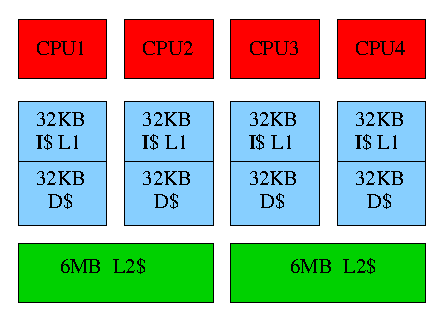
\includegraphics[width=6cm,height=8cm, keepaspectratio]{images/Xeon.eps}} \qquad\qquad
 \subfigure[Machine B: Intel i7 870 \label{fig:i7}]%
  {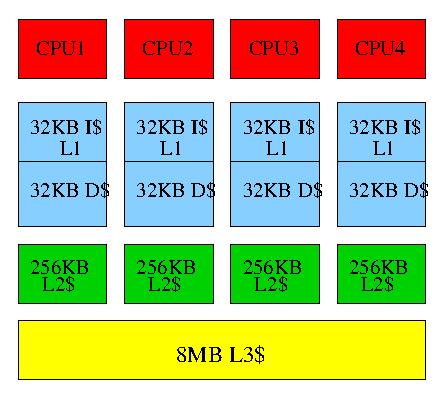
\includegraphics[width=6cm,height=8cm, keepaspectratio]{images/i7.eps}}
 \caption{\figurecaption{Cache configurations on computers used in this work. Those with D\$ are data cache, those with I\$ are instruction caches and 
the others are unified, that is, cache serves to data and instructions.
 }}
\end{figure}

\begin{description}
\item[Machine A] The first machine is an Intel Xeon E5440 running at 2.83GHz. There is not any cache shared among all cores. The LLC consists in two 
big L2-caches, of 6MB each, shared between sets of 2 cores cache hierarchy is shown in Fig. \ref{fig:Xeon}. On this machine there are two dies: CPU0 and 
CPU1 are on the same die, while other CPUs are on other die.

\item[Machine B] The second machine is an Intel Core i7 870 processor. It runs at 2.93 GHz and has the cache configuration as illustrated in Fig. 
\ref{fig:i7}. The LLC consists in one L3 of 8MB, which is shared by all cores. The L2-caches are private to each processor. All CPUs are on the same die.

\end{description}

The Benchmark used is the same as used in master thesis \cite{lcs}, in Fig.\ref{fig:bench} is represented its structure.

\begin{figure}[htbp]
\centering
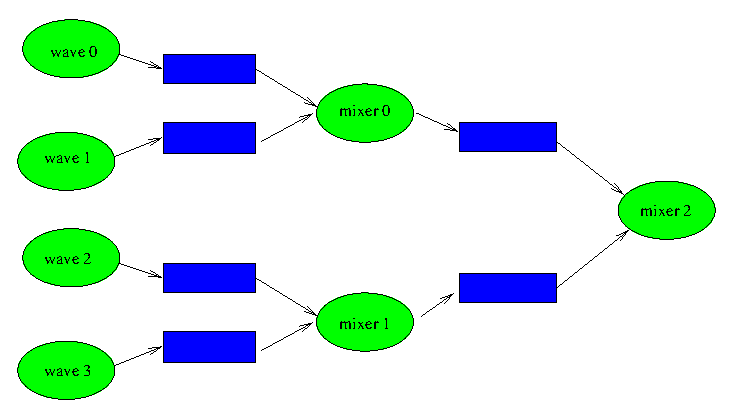
\includegraphics[width=\widefigure]{images/bench.eps}
\caption{\figurecaption{Structure of benchmark used: task are green coloured, buffer are blue coloured}}
\label{fig:bench}
\end{figure}

The Execution of benchmark is divided in three steps:

\begin{enumerate}
\item Waves write their buffer
\item Mixers read data from two buffers filled by waves, they mix read data and write them on their buffer, for example \textit{mixer0} reads data 
from the buffer filled by \textit{wave0} and from the buffer filled by wave1, mixes the data and then writes its buffer.
\item The Last mixer, reads data from the buffers written by \textit{mixer0} and \textit{mixer1}, mixes the data and writes its buffer.
\end{enumerate}

When \textit{mixer2} has finished to write data on its buffer, we say that a \textit{sample} was produced. The execution time to produce a sample 
depends on the buffers dimension, because each task has to fill its buffer. Note that waves fill their buffers with integers of 2 byte, therefore if 
buffer is of 4KB they will write 2048 integers in their buffer. Buffer dimension is always a power of 2.
The metric used to evaluate benchmark performance is the same as used in \cite{lcs}: 
\begin{equation}
	average + 2*standard deviation (A2S), 
\label{eq:metric_rt}
\end{equation}

where \textit{average} is the average of execution time to produce a sample and \textit{standard deviation} is the standard deviation of execution 
time to produce a sample. With this metric is possible measure throughput and predictability of the application.

%%%%%%%%%%%%%%%%%%%%%%%%%%%%%%%%%%%%%%%%%%%%%%%%%%%%%%%%%%%%%%%%%%%%%%%%%%%%%
\section{Analysis of Taskaffinity behaviour}

This section analyzes which are the improvements and downsides that the current version of task-affinity shows on different test computers and various
buffer dimensions.

In the following experiments only the Intel Xeon and Intel i7 architectures are considered, because their cache architectures are similar in structure.
These architectures differing in inter-chip communication, the former uses Quick-path Interconnect (QPI) the latter uses Hyper-transport (HT). 
Furthermore, Intel i7 uses an inclusive LLC with MESIF protocol. To observe how these factors impact on task-affinity a complex analysis would be required 
and this is not the goal of this thesis.
 
%-----------------------------------------------------------------------------
\subsection{Application's performance}

The length of the buffers determine how long the work executed by producers and consumers takes. It was showed in \cite{lcs} that if buffers used are 
too short and consequently tasks have very few work to do in user-space side, the parallelism provided by the SMP system is not well profited. For 
this reason, in \cite{lcs} a buffer of 4KB was used, in this way, parallelism was well profited. In the following graphics, we compare vanilla and 
current version of task-affinity in terms of predictability and throughput on different architectures and using different buffer dimensions.

\begin{figure}[htbp]
\centering
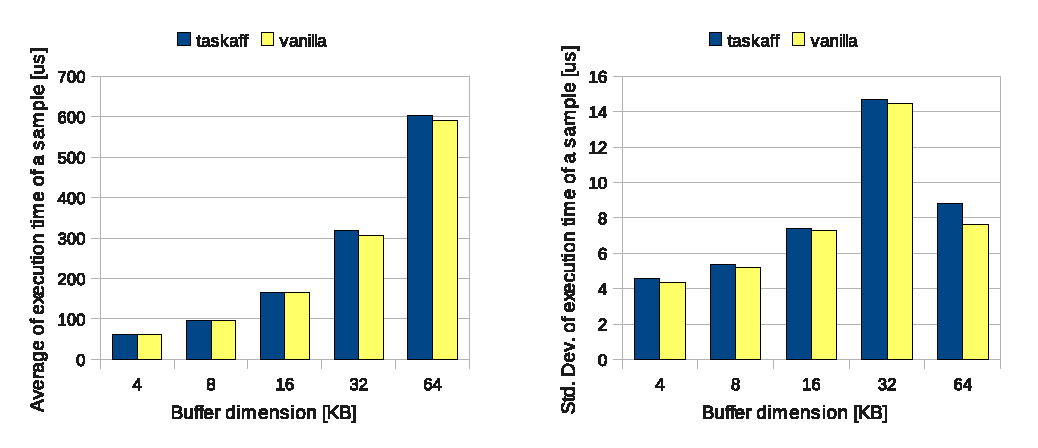
\includegraphics[width=\widefigure]{images/time/time_avg_var_Xeon.eps}
\caption{\figurecaption{Average and Std. Deviation of execution time of a sample on Xeon}}
\label{fig:avg_var_xeon}
\end{figure}

\newpage

\begin{figure}[htbp]
\centering
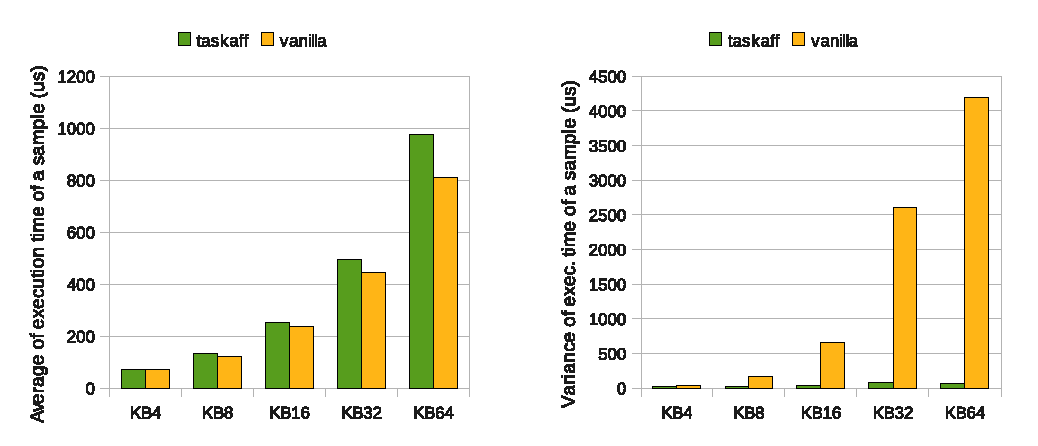
\includegraphics[width=\widefigure]{images/time/time_avg_var_i7.eps}
\caption{\figurecaption{Average and Std. Deviation of execution time of a sample on i7}}
\label{fig:avg_var_i7}
\end{figure}

\begin{table}[htbp]
\begin{center}
\begin{tabular}{|l|c|c|c|}
	\hline
	       & \multicolumn{2}{|c|}{Speedup} \\ 
	       & Xeon    & i7     \\ \hline
	$4KB$  & -1.89\% & 2.33\% \\ \hline
	$8KB$  & -0.82\% & 6.42\% \\ \hline
	$16KB$ & -0.31\% & 8.42\% \\ \hline
	$32KB$ & -3.96\% & 6.53\% \\ \hline
	$64KB$ & -3.25\% & -5.14\% \\ \hline
\end{tabular}
\caption{Speedup obtained with task-affinity on different architectures with different buffer}
\label{tab:speedup_xeon_i7}
\end{center}
\end{table}

Speedup on Table \ref{tab:speedup_xeon_i7} is calculated in this way:

\begin{equation}
        \frac{A2S_{task\_affinity} - A2S_{vanilla}}{A2S_{vanilla}}
\label{eq:miss_rate}
\end{equation}

Where $A2S_{task\_affinity}$ and $A2S_{vanilla}$ are calculated using \ref{eq:metric_rt}.

As shown in graphics and as summarized in Table \ref{tab:speedup_xeon_i7}, the current version of task-affinity is not effective on Intel Xeon.
In terms of throughput task-affinity is not better than vanilla, because the average of execution time of a sample is about the same in both kernels 
and this is true for both the architectures. In term of predictability, on Intel i7, task-affinity is better than vanilla, especially with buffer 
greater than 32KB. Task-affinity should reduce both L1 and LLC cache misses and, consequently, improve predictability of application. But this fact 
doesn't occur on Intel Xeon. In Fig. \ref{fig:l1_load_store_Xeon} and \ref{fig:l1_load_store_i7} we can see respectively L1 read and write misses on 
Xeon and i7.

\begin{figure}[htbp]
 \centering
  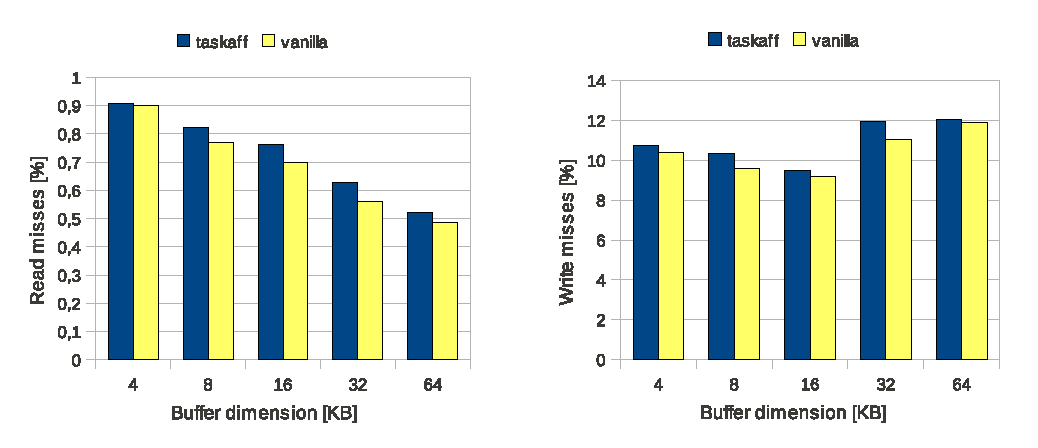
\includegraphics[width=\widefigure]{images/cache_miss/l1_load_store_Xeon.eps}
  \label{fig:l1_load_store_Xeon}
 \caption{\figurecaption{L1 miss rate of read and write instructions on Xeon}}
\end{figure}

\begin{figure}[htbp]
 \centering
  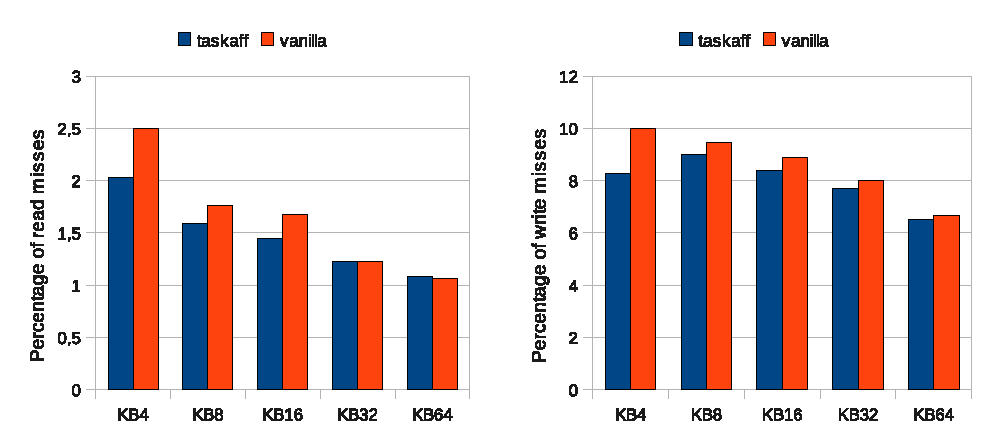
\includegraphics[width=\widefigure]{images/cache_miss/l1_load_store_i7.eps}
  \label{fig:l1_load_store_i7}
 \caption{\figurecaption{L1 miss rate of read and write instructions on i7}}
\end{figure}

On Intel Xeon read and write miss rates are increased and, consequently, predictability is degradated.

%-----------------------------------------------------------------------------
\subsection{Impact of task migration on execution time predictability}

Migration of tasks is an important factor that influences cache misses. Current version of task-affinity is not very effective in terms of reduction 
of task's migrations. As already described in \cite{lcs}, during the benchmark's execution, \textit{mixer0} or \textit{mixer1} bounce between two 
different CPUs. This issue is not related to the architecture or the buffer dimension, but it is related to the logic of task-affinity. To understand 
the reason of this problem see Fig. \ref{fig:migr_pat}.

\begin{figure}[h]
\centering
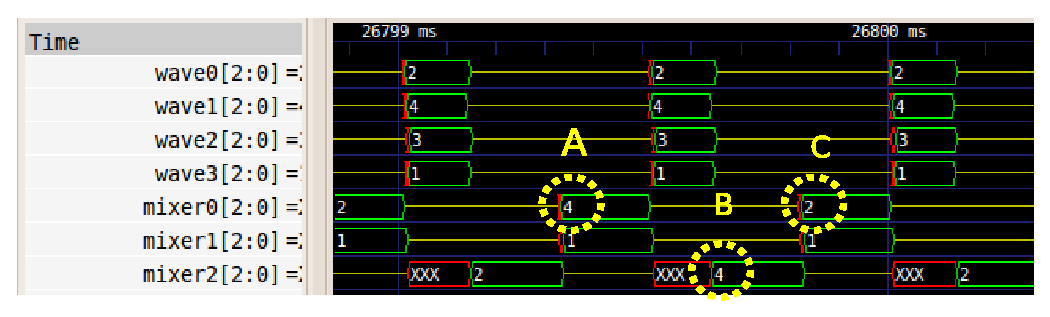
\includegraphics[width=\widefigure]{images/migr_i7.eps}
\caption{\figurecaption{Step A: \textit{mixer0} chooses CPU4. Step B:
\textit{mixer2} chooses CPU4. Step C: mixer0 chooses CPU2}}
\label{fig:migr_pat}
\end{figure}

This picture was made using \textit{gtkwave}, a tool that show in a graphic way the scheduling performed.
Consider step A. According to the current task-affinty logic, \textit{mixer0}
has to choose a CPU that has executed \textit{wave0} or 
\textit{wave1}, that is CPU2 or CPU4, \textit{mixer2} has to choose a CPU that have executed \textit{mixer0} or \textit{mixer1}, that is CPU3 or 
CPU1. \textit{mixer0} chooses the least loaded runqueue, therefore it chooses CPU4. At Step B \textit{mixer2} can choose between CPU4 or CPU1, they 
have the same number of Real-time task, therefore \textit{mixer2} choose the
first CPU in its list, that is CPU4. At step C, \textit{mixer0} has to 
choose CPU2 or CPU4 again, but it can't choose CPU4, as in step A, because it is still occupied by \textit{mixer2}, so \textit{mixer0} has to be 
executed on CPU2. This is the problem. Since \textit{mixer0} or \textit{mixer1}
choose a CPU occupied by \textit{mixer2}, one of them will have to migrate.

Task's migration can degrade performance because a migrated task could warm up a new cache and it could create new cache interference in a new 
location already occupied by other tasks. In order to measure how much this migration pattern increases miss rate of the application, the following 
experiment was performed: two run of the benchmark are performed, in the first
run all tasks are pinned on a specific CPU and they can't migrate, in 
the second run only waves are pinned and mixers can migrate,
Tab.\ref{tab:assignment} summarizes the relative CPU assignments. 

\begin{table}[tbp]
\centering%
\subfigure[All task pinned]{%
 \begin{tabular}{c|c}
	\hline
	Task & CPU \\ \hline
	Wave0 & 1  \\ \hline
	Wave1 & 2 \\ \hline
	Wave2 & 3 \\ \hline
	Wave3 & 4 \\ \hline
	Mixer0 & 1 \\ \hline
	Mixer1 & 3 \\ \hline
	Mixer2 & 3 \\ \hline
 \end{tabular} 
 \label{tab:all_pinned}
}\hspace{4em}
\subfigure[Waves pinned]{%
 \begin{tabular}{c|c}
	\hline
	Task & CPU \\ \hline
	Wave0 & 1  \\ \hline
	Wave1 & 2 \\ \hline
	Wave2 & 3 \\ \hline
	Wave3 & 4 \\ \hline
 \end{tabular} 
 \label{tab:cpuaff_waves}
}
\label{tab:assignment}
\caption{CPUs assignment}
\end{table}

What we expect with all tasks pinned and with buffer less than 32KB is a decrease of L1 read and write miss rates and a reduction of accesses to LLC. 
With dimensions greater than 32KB, the buffers can't be loaded entirely in L1 cache, therefore we don't know effect on L1 miss rates. Anyway LLC miss 
rates should diminish. With buffer less than 32KB, accesses to LLC are very different between cases with all task pinned and case with only waves 
pinned and then, miss rates that occur in two cases are not longer comparable. Note that on Intel i7, LLC is L3 and between L1 and L3 there are private L2 
caches that can store buffer of 32KB and 64KB, therefore also with buffers of 32KB and 64KB accesses to LLC should be very different in the considered cases.
But as we will see in the following graphics, also on Intel i7, in the
considered cases, the number of accesses to LLC is about the same with buffer greater 
than 32KB. 

\begin{figure}[htbp]
\centering
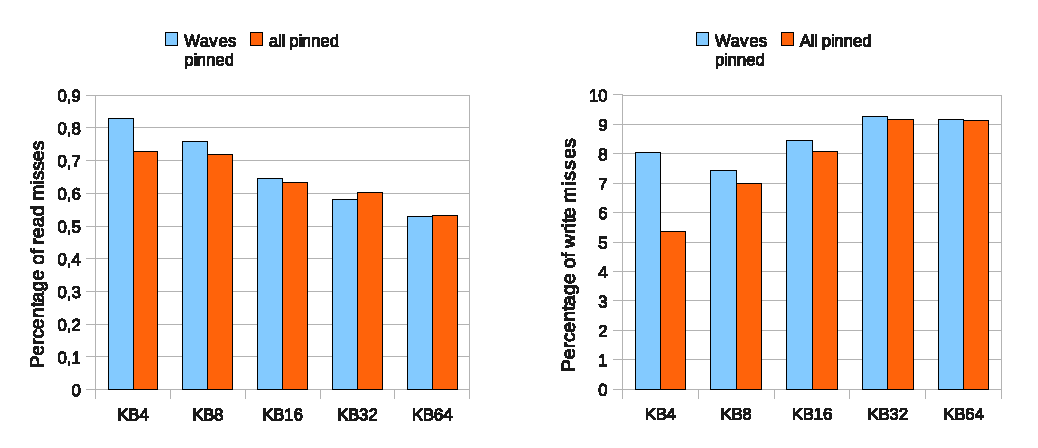
\includegraphics[width=\widefigure]{images/cpuaff/cpuaff_l1_load_store_Xeon.eps}
\caption{\figurecaption{L1 miss rate of read and write instructions on Xeon}}
\label{fig:cpuaff_l1_load_store_xeon}
\end{figure}

\begin{figure}[htbp]
\centering
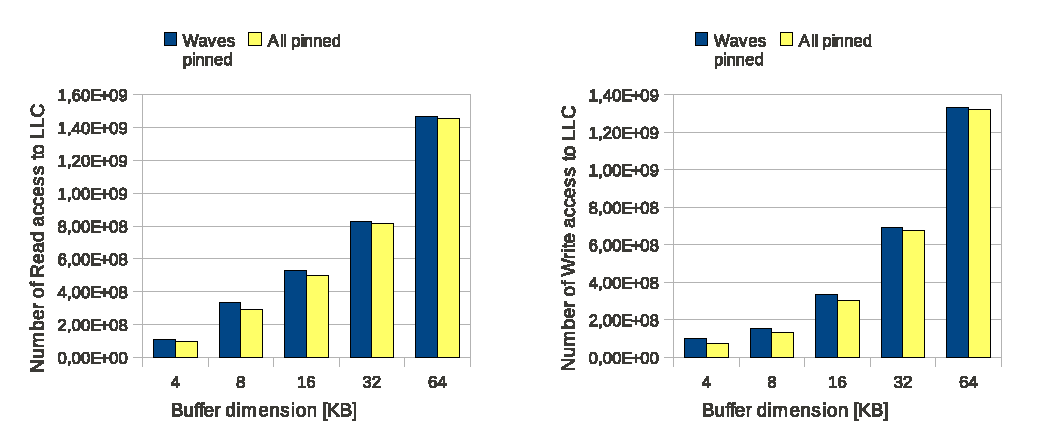
\includegraphics[width=\widefigure]{images/cpuaff/cpuaff_acc_l2_load_store_Xeon.eps}
\caption{\figurecaption{Number of LLC read and write accesses on Xeon}}
\label{fig:cpuaff_acc_l2_load_store_xeon}
\end{figure}

\begin{figure}[htbp]
\centering
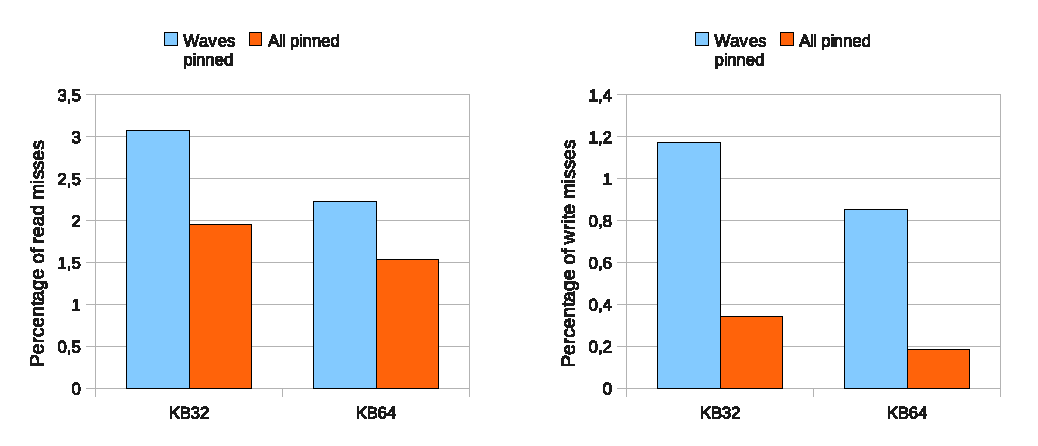
\includegraphics[width=\widefigure]{images/cpuaff/cpuaff_l2_load_store_Xeon.eps}
\caption{\figurecaption{LLC miss rate of read and write instructions on Xeon}}
\label{fig:cpuaff_l2_load_store_xeon}
\end{figure}
\newpage

\begin{figure}[htbp]
\centering
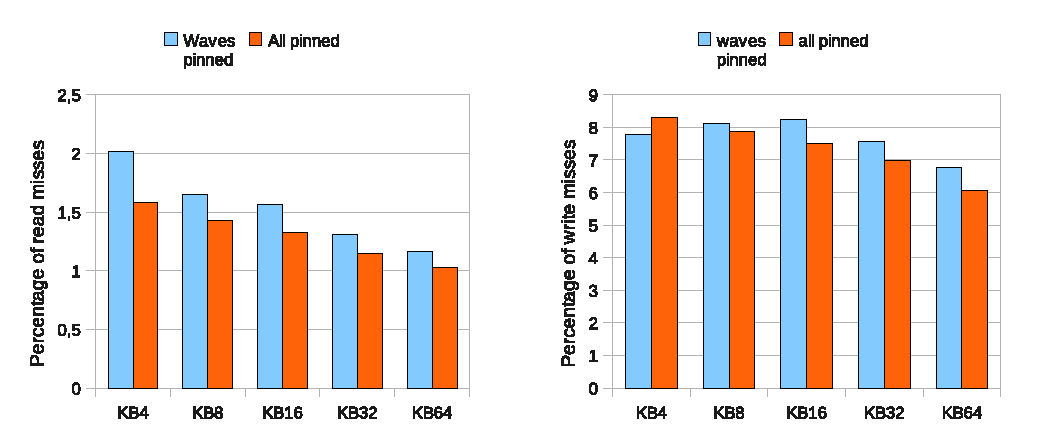
\includegraphics[width=\widefigure]{images/cpuaff/cpuaff_l1_load_store_i7.eps}
\caption{\figurecaption{L1 miss rate of read and write instructions on i7}}
\label{fig:cpuaff_l1_load_i7}
\end{figure}

\begin{figure}[htbp]
\centering
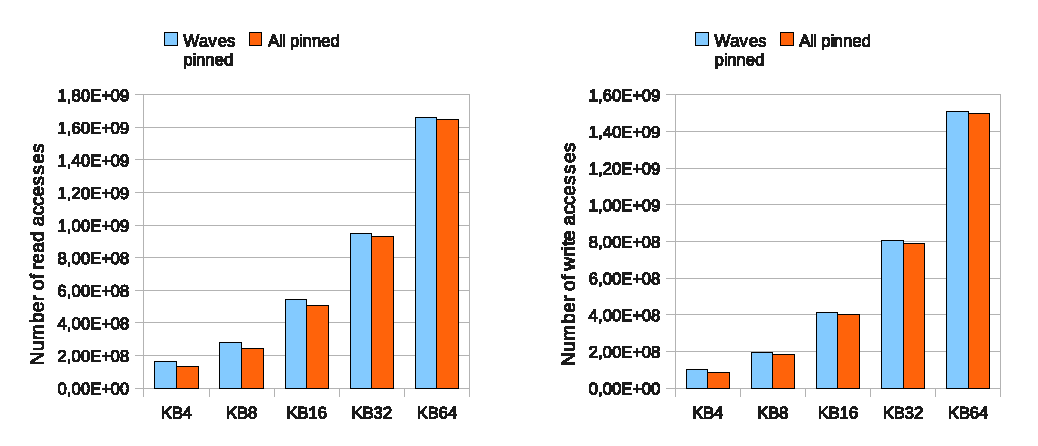
\includegraphics[width=\widefigure]{images/cpuaff/cpuaff_acc_l3_load_store_i7.eps}
\caption{\figurecaption{Number of LLC read and write accesses on i7}}
\label{fig:cpuaff_acc_l2_load_store_i7}
\end{figure}

\begin{figure}[htbp]
\centering
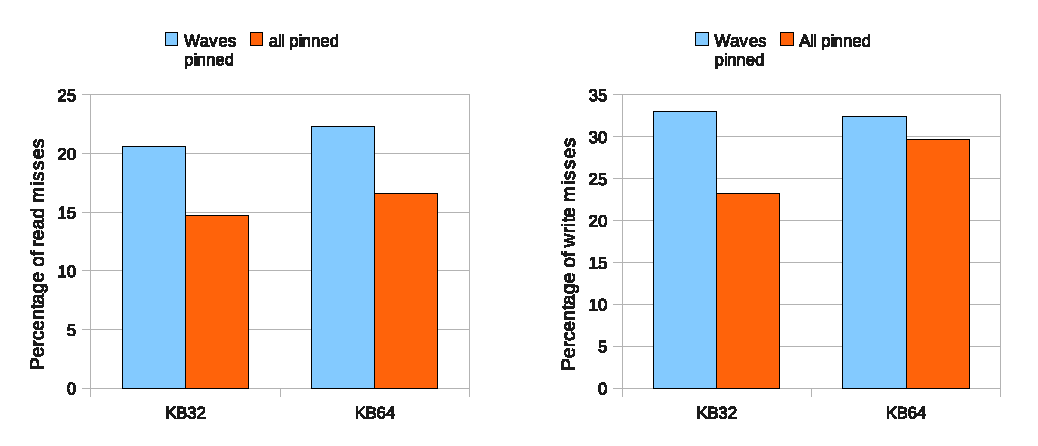
\includegraphics[width=\widefigure]{images/cpuaff/cpuaff_l3_load_store_i7.eps}
\caption{\figurecaption{LLC miss rate of read and write instructions on i7}}
\label{fig:cpuaff_l1_load_i7}
\end{figure}

\newpage
%-----------------------------------------------------------------------
\subsection{Considerations on experimental results}

We can infer from these graphics, that migration pattern have a great influence on read/write miss rate on LLC in both architectures considered. 

On Intel Xeon, L1 and LLC read and in particular write misses are greatly increased, this fact is due to cache architecture. On Xeon cores are not all on 
the same die, for example: assume that core 1 and 2 are on the same die, while core 3 and 4 are on the other die. If a task is executed on core 1 and 
request a data on core 3, that request will result in a miss, therefore if a task bounces from CPUs that own to different dies, each time it has to warm 
up the cache. This issue regards especially write operations, because for read operations, hardware prefetchers mitigate this problem.

On Intel i7, instead all core share a common LLC. When a core requires a data, it sends a data request to L3 cache. If data is in L3 and there is a hit, 
the L3 cache query the "core valid" bits of the cache line that contains requested data, in order to know which is the core that owns requested data. The 
core that owns requested data reply to the request with the most recent copy of data. For this reason, each core on i7 can use data in other private cache
because all data are contained in LLC.

To get a sense on how much cache miss influence predictability of the application, see Fig. \ref{fig:time_cpf_var_Xeon_i7}. In the graphics two run of the
benchmark are compared: in the first run all tasks are pinned, while in the second run all tasks can migrate according migration policy of vanilla kernel.

\begin{figure}[htbp]
\centering
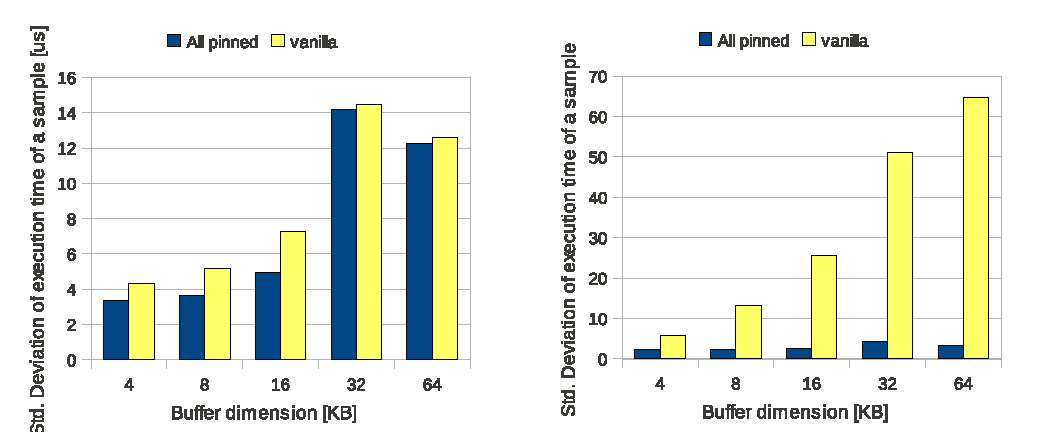
\includegraphics[width=\widefigure]{images/cpf_time/time_cpf_var_Xeon_i7.eps}
\caption{\figurecaption{Std. Deviation of execution time of a sample on Xeon and i7: all task pinned compared vanilla}}
\label{fig:time_cpf_var_Xeon_i7}
\end{figure}

It is interesting to note how the absence of migration improve the predictability when buffer used are greater than 32KB that can't be stored in L1 but 
only in LLC cache or in private L2 (Intel i7).

Performance degradation on Intel Xeon is not only due to migration pattern. As I said before, cache architectures of Xeon and i7 are very different and
from previous graphics seems that with cache architecture of Intel i7, task-affinity is more effective, but there is another important aspect that 
influences performace: it is \textbf{Inter-chip communication}. Intel i7 use the new Quick-path Interconnect that is a point-to-point processor 
interconnect developed by Intel to compete with HyperTransport. This first implementation of this bus achieve 25.6 GB/s, which provides exactly double the 
theoretical bandwidth of Intel's 1600 MHz FSB, that is the best performance obtainable with FSB. From datasheet, Intel Xeon E5440 use a FSB at 1333 MHz, 
therefore communication between chips are more faster on i7. Hence, it is clear that communication between cores that belong to different dies is very 
expensive on Intel Xeon. On Intel Xeon, \textit{mixer0} or \textit{mixer1} could find one buffer in L1 cache and other buffer in a bank of L2 that is 
shared by the CPU that have execute it. \textit{Mixer2} could find one buffer on L1 one cache, while other buffer is \textit{always} placed on bank of L2 
that is not shared by the cpu that has executed \textit{Mixer2}, therefore read latencies are very high, because data are placed on different dies. 
On i7, instead, \textit{mixer2} could find one buffer in L1 cache and other buffer in L3 cache that is shared among all cores and it is inclusive, 
therefore to read data is less expensive on i7.

%%%%%%%%%%%%%%%%%%%%%%%%%%%%%%%%%%%%%%%%%%%%%%%%%%%%%%%%%%%%%%%%%%%%%%%%%%%%%
\section{Task-affinity improvements}

Before to explain how the new kernel patch works, it is necessary to remember the concept of task-affinity. We say that two tasks have a task-affinity 
relationship if they share data and their execution depends upon reading or writing this data \cite{lcs}. In a producer-consumer application, the 
producer is the one that writes to the shared buffer, while the consumer is the one that reads it. The consumer depends on data generated by the producer 
since it needs it in order to be able to run, therefore we say that the consumer has a task-affinity relationship toward the producer.

\begin{figure}[htbp]
\centering
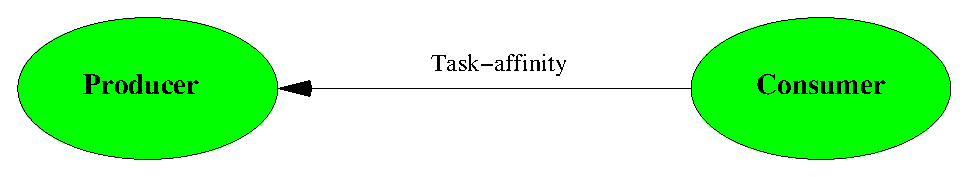
\includegraphics[width=\widefigure]{images/taskaff-rel.eps}
\caption{\figurecaption{Task-affinity relationship between producer and consumer}}
\label{fig:taskaff-rel}
\end{figure}

Each task is provided with a linked list called \textit{taskaffinity\_list} that contains all tasks to which it has task-affinity relationship, briefly 
all its producers. To insert and delete a task in a \textit{taskaffinity\_list} two new system calls are provided:

\begin{description}

\item[sched\_add\_taskaffinity:] This system call adds a dependency to the current task, i.e. the task that issued the call. It receives, as parameter, the 
pid of the task the current one will be dependent upon.

\item[sched\_del\_taskaffinity:] When a task does not want anymore to use the task-affinity mechanism, it is possible to remove it through this call.
As in the case of inclusion of dependency, it suffices to pass as parameter the pid of the task one wants not to follow anymore.

\end{description}

Thanks to these system calls, the scheduler "knows" which tasks have task-affinity and, in this way, it can schedule consumers after producers in order to 
enforce reuse of cache memory.

The task-affinity logic influences wake up and migration of a task. As we have
previously seen, in \textit{try\_to\_wake\_up} the choice of CPU where to 
put the to be waken task is made by \texttt{select\_task\_rq\_rt} \ref{code:select_task}. This function is modified in this way: given the input task $p$, 
the function doesn't call \texttt{find\_lowest\_rq} but it loops for all element present in the $p$'s \textit{taskaffinity list} and build a mask, called 
\textit{affinity\_mask}, with CPUs that have executed a task present in $p$'s
\textit{taskaffinity\_list}. Finished the loop, the function returns the CPU 
with the runqueue that has the lowest number of Real-Time tasks. Only if the
mask is empty, the function calls \texttt{find\_lowest\_rq} to choose a CPU
in the standard way. 

In the current version of task-affinity, a task that "respect" task-affinity, that is a task that was enqueued according to its task-affinity 
relationships, isn't able to migrate. In plain words, \texttt{push\_rt\_task} and \texttt{pull\_rt\_task} can't move tasks that "respect" task-affinity.

The aim of this policy is clear: when a task wakes up, the policy tries to
select the best CPU for that task and, if it finds it, it blocks the task on the 
best runqueue until the task's execution. For this reason the key point of this task-affinity logic is the \texttt{select\_task\_rq\_rt}. In the optimal 
case, producers and consumers will be executed subsequently always on the same
CPU.

Nevertheless, in practice, the chosen CPU for $p$ is next to never the optimal
CPU. The reason is very simple. The choice of the best 
CPU, and the enqueuing of task are performed in different moments. When \texttt{select\_task\_rq\_rt} is called, it doesn't hold any lock. During the loop, 
the function has to read what is the content of different runqueues present in
the system, these reads are not synchronized. Once the CPU is selected, 
\texttt{select\_task\_rq\_rt} returns and \texttt{try\_to\_wake\_up} \textbf{takes a lock} on the chosen runqueue, in order to call 
\texttt{activate\_task} to perform the enqueuing of the task. From when
\texttt{select\_task\_rq\_rt} selects the CPU to when the lock is taken, a task 
with equal or higher priority than $p$'s priority can be inserted in the selected runqueue and, in this way, the next task that will be executed won't be 
$p$. 

The current version of task-affinity ensures only weak concept of temporal locality because it doesn't ensure, when it is possible, that the next task 
executed after a producer is a consumer. Another problem of the current version of task-affinity is the migration policy. It is not very flexible. Pull 
and push functions maintain the system balanced, and guarantee that every CPU executes always the higher priority Real-time task present in its runqueue.
Therefore, the denial to pull and push can improve predictability of the application and can degrade significantly the throughput of the application.
Predictability is an important aspect for Real-time systems, but if we have a very bad throughput we don't exploit the potentiality of multicore platforms.

The aim of the patch developed in this thesis is to improve the concept of temporal locality in order to execute a consumer immediately after a 
producer, when it is possible and to improve the migration policy in order to use also the functions involved in the migration mechanism to exploit the 
concept of task-affinity. Furthermore, the patch makes task-affinity more robust synchronizing the accesses to data structures used. With this patch we 
try to improve throughput and predictability of the application. 

%%%%%%%%%%%%%%%%%%%%%%%%%%%%%%%%%%%%%%%%%%%%%%%%%%%%%%%%%%%%%%%%%%%%%%%%%%%%%
\section{Patch structure}

The proposed patch is divided in two parts. The first part improves the temporal locality, while the second part introduces mechanisms to synchronize 
accesses to task-affinity data structures.

%-----------------------------------------------------------------------------
\subsection{Temporal locality}

The implemented logic to improve temporal locality is divided in the following parts:

\begin{description}

\item[last\_tsk field] To ensure that a consumer will be the next executed task after a producer, it is necessary to change what 
\texttt{select\_task\_rq\_rt} "sees". As I previously said, during its loop, \texttt{select\_task\_rq\_rt} checks for CPUs that \textbf{have executed} a 
task in $p$'s \textit{taskaffinity list}. It means that, in that moment, those
CPUs could be executing a task that is not a producer and such, the L1 cache 
could already be dirty. For this reason, at each runqueue was added a field named \texttt{last\_tsk} that contains the last task executed in a runqueue. 
This field is updated at each context switch if the next task to be executed is different from idle. In this way, if current task on runqueue is not idle, 
this field represents, the task in execution. With this additional field, \texttt{select\_task\_rq\_rt} "knows" which is the task currently executing on 
each runqueue. In this way, CPUs that during \texttt{select\_task\_rq\_rt} are executing a task that is not in $p$'s \textit{taskaffinity\_list} are not 
inserted in \texttt{affinity\_mask}.

\item[enqueue on head] This change is not enough. Consider this situation: two
different CPUs that we call CPU\_A and CPU\_B are executing two different 
instances of \texttt{try\_to\_wake\_up}. Respectively, they are called for task $p$ and task $q$: the former has task-affinity relationship, the latter is 
a generic Real-time task, both tasks have the same priority. Suppose that the current task on CPU\_A is a task in $p$'s \textit{taskaffinity list} and then 
\texttt{select\_task\_rq\_rt} choose CPU\_A for $p$. Suppose that \texttt{try\_to\_wake\_up} that wakes up $q$ chooses CPU\_A and enqueue task $q$ on the 
runqueue of CPU\_A. Task $p$ is not yet enqueued, therefore when it will be enqueued, it will be preceded by $q$ and then the next task that will
be executed on CPU\_A is $q$.

\begin{figure}[htbp]
\centering
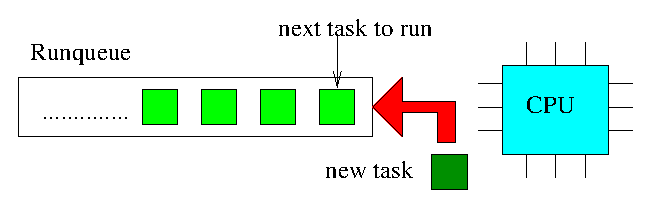
\includegraphics[width=10cm,height=12cm, keepaspectratio]{images/enq_head.eps}
%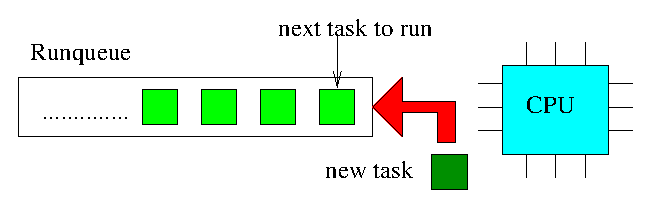
\includegraphics[width=\widefigure]{images/enq_head.eps}
\caption{\figurecaption{Enqueue on head}}
\label{fig:enq_head}
\end{figure}

To resolve this problem a task that "respects" task-affinity is enqueued on the top of a runqueue and not on its tail. In this way, if two Real-time tasks 
are on the same runqueue and have the same priority, but one of them "respects" a task-affinity, the next task that will be executed is the task that 
"respects" a task-affinity. 

\item[choice of current task] Even if a task with task-affinity is enqueued on head in a runqueue, it will be the next executed task only if it is 
enqueued before it is executed a task that is already on that runqueue. For this reason, it is necessary to optimize the choice made in 
\textit{select\_task\_rq\_rt}. In \texttt{select\_task\_rq\_rt}, when a task with task-affinity, that we call $p$, has built its \textit{affinity mask}, 
it checks if in that mask there is the CPU that is executing the \texttt{try\_to\_wake\_up} that are waking up it. If this is true, it means that the 
current task on that CPU is a $p$'s producer and now on that CPU a \texttt{try\_to\_wake\_up} is in execution, therefore any other task enqueued on that 
CPU in that moment can't be executed, because during \texttt{try\_to\_wake\_up} kernel preemption is disabled and then it is necessary wait that 
\texttt{try\_to\_wake\_up} finish. Choosing that CPU, $p$ will be the next task executed on that CPU, because it is enqueued on head and it can precede 
all task enqueued on that CPU during \textit{select\_task\_rq\_rt}.

\item[migration mechanism] There is another a problem. It could happen that a task with higher priority is enqueued on the same runqueue where a task with 
task-affinity is enqueued. In this case, the next task to execute won't be the task with task-affinity.
To resolve this problem, migration mechanism is used. When the \texttt{try\_to\_wake\_up} has enqueued task $p$ it calls function \texttt{task\_woken} in 
order to checks if $p$ can be immediately executed on the selected runqueue or not. If on the runqueue there is a task with priority equal or higher than 
the $p$'s priority and this task precedes $p$, \texttt{push\_rt\_task} is called
and $p$ can be pushed on another CPU. To select the CPU where to push $p$, 
the same mechanism used in \texttt{select\_task\_rq\_rt} is adopted. Therefore, $p$ will be pushed where it is in execution a task in $p$'s 
\textit{taskaffinity\_list}, if it is impossible standard push criteria are
adopted and $p$ will be pushed on a CPU that executing a task with lower 
priority than $p$. Obviously, in order to push a task that "respect" task-affinity, it is necessary insert it in a \textit{pushable list}. 

\end{description}
%-----------------------------------------------------------------------------
\subsection{Synchronization}

In the current version of task-affinity, accesses to data structures used to manage task-affinity are made by user or by kernel. The resource that must be
synchronized is \texttt{taskaffinity\_list}

\begin{description}

\item[Access from user space:] the user space can access task-affinity data structures using syscalls \texttt{sched\_add\_taskaffinity}, and 
\texttt{sched\_del\_taskaffinity}. These functions access the pid of the task received in input in synchronized way, by using the read-write lock
tasklist\_lock that protects the kernel's internal task list. For this reason, at every moment, only one instance of these syscalls can modify the
task-affinity data structure of a task.

\item[Access from kernel space:] here the situation is more complex. There are two functions that can access to task-affinity data structures, they are:\\
\texttt{task\_affinity\_notify\_exit} and \texttt{select\_task\_rq\_rt}. The former function frees task-affinity data structures and is called when a 
task is exiting. During this phase, all resources used by a task, pid included, are deallocated. Therefore, when \texttt{task\_affinity\_notify\_exit} is 
called, \textit{tasklist\_lock} is acquired. This is not enough because in that moment \texttt{select\_task\_rq\_rt} could access the task-affinity data 
structures of the exiting task, for this reason another layer of synchronization is needed. To resolve this problem, each task has its own read-write lock 
named \textit{taskaff\_lock} to protect its task-affinity data structures. 

\end{description}



\cleardoublepage
\chapter{Experimental Results}
\label{cha:exper_results}


\cleardoublepage
\chapter{Conclusions and future developments}
\label{cha:ConclusionsFutureDev}

In this work we have investigated behaviour of task-affinity on different architectures. Task-affinity is based on assumption that, if tasks share a great 
amount of data and we have an SMP architecture, then occasionally executing them on the first available processors will increase the cache-miss rate. If we 
move tasks to be executed near to where data was produced, then we spare some cache-misses \cite{lcs}. We have demonstrate that this assumption is not 
always true. Migrations of tasks play an important role on predictability of the applications. When a task migrates, data could be moved from one cache to 
another. As we have seen on Intel Xeon and as it is demonstrated in \cite{molka}, this operation may involve high latency that depends on cache 
architecture, inter-chip communications and other hardware factors. Therefore it is clear that it is not enough to execute tasks that share common data 
on the same CPUs, but it is necessary guarantee that tasks that share common data find what they need possibly in L1 cache. For this reason, we have 
improved the concept of temporal locality.

The experimental results show that task-affinity is effective on Intel i7, where there is an average speedup in term of A2S of $\sim 17\%$. We have 
increased task migration, nevertheless we have improved throughput and predictability. It is clear that architecture of Intel i7 mitigates the side effects 
of the high number of migrations of tasks. On Intel Xeon task-affinity is effective only with buffer greater than 4KB, in that case there is an average 
speedup in term of A2S of $\sim 10,5\%$. It is clear that the effect of migrations of tasks is more significant on this architecture.

We could obtain results still better with a more effective migration policy. In this patch, in order to improve the temporal locality, we have included 
\textit{push\_rt\_task} in the task-affinity logic and we have seen that, because of the scheduling performed, \textit{pull\_rt\_task} has an higer overhead
than vanilla. 

We conclude that the mechanism proposed brought, in fact, an improvement of throughput and on determinism of the entire application, especially with buffers
of big dimension as 32KB. It is interesting that these improvements take place even if L1 and LLC miss rates increase (Intel Xeon) therefore it is clear
that, according to the cache architecture used, cache misses have a different impact on performance of application.


%%%%%%%%%%%%%%%%%%%%%%%%%%%%%%%%%%%%%%%%%%%%%%%%%%%%%%%%%%%%%%%%%%%%%%%
\section{Future Works}

During the development of task-affinity, NUMA architectures were never considered. In the final part of this thesis we have started to analyze the 
behaviour of task-affinity on AMD Opteron, a NUMA architecture. In a first trial, using some kernel facilities, we have held all tasks to be executed only 
on one node, in order to simulate an SMP architecture. We have obtained the following results:

\begin{figure}[htbp]
\centering
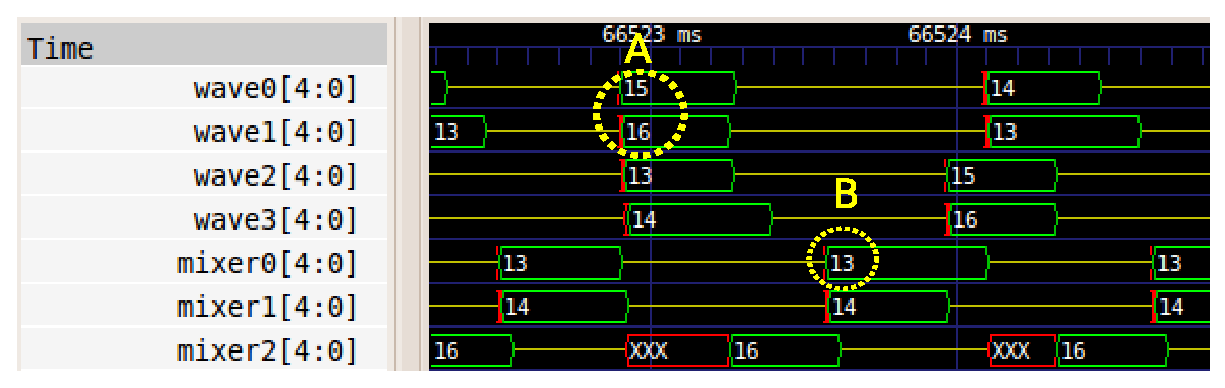
\includegraphics[width=\widefigure]{images/results_AMD/final_AMD.eps}
\caption{\figurecaption{Scheduling performed by task-affinity on Opteron}}
\label{fig:trace_AMD}
\end{figure}

\begin{figure}[htbp]
\centering
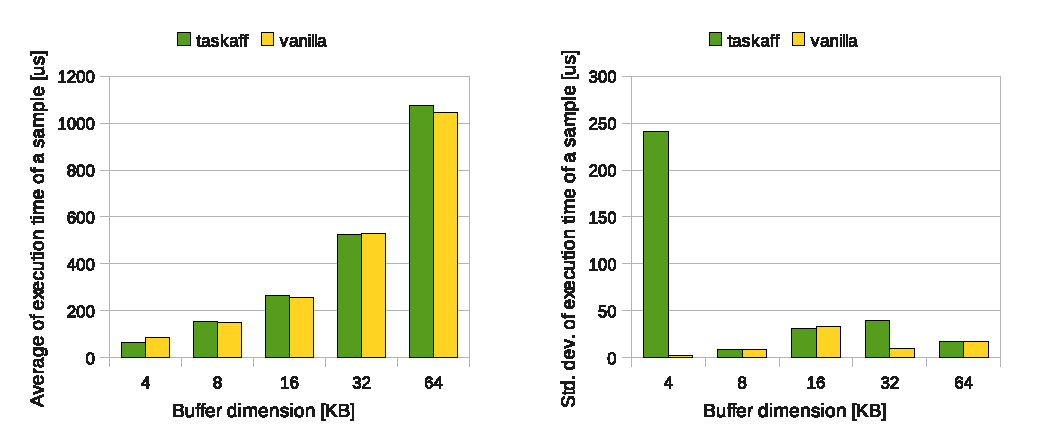
\includegraphics[width=\widefigure]{images/results_AMD/time_avg_var_AMD.eps}
\caption{\figurecaption{Average and Variance of execution time of a sample Opteron}}
\label{fig:time_avg_var_AMD}
\end{figure}

Task-affinity on this machine doesn't work properly. We can see in step B that \textit{mixer0} doesn't choose the correct CPU. The incorrect behaviour of 
task-affinity is also reflected by Fig. \ref{fig:time_avg_var_AMD}, where we can see a worsening of throughput and predictability. It is possible that the 
task-affinity doesn't work, because of a lot of kernel threads used to manage load balancing and others kernel activities in NUMA architectures: but this is 
only an hypotesis. According these results, it is clear that task-affinity needs the support for NUMA architectures, this is the first step to improve 
task-affinity.

In this work, we have seen that cache misses have a different impact on determinism of application on different architectures, it is necessary to 
estimate how much cache misses impact on application performance and in particular on determinism, in order to understand if the task-affinity could 
improve significantly or not the determinism of application on a given architecture. 

Another possible improvement is to optimize the migration policy, in order to include also \textit{pull\_rt\_task} in task-affinity logic and finally, it 
would be better not to use system calls to define dependencies among tasks, but, instead, to rely in other mechanisms, such as a profiler \cite{calandro}, 
that infers automatically the dependencies among tasks. The reason is that it is not desirable to modify present applications to use the task-affinity. 
The mechanism of adding and removing dependencies would be rather the same: only the user interface would need to be changed.


\newpage

\cleardoublepage
\chapter{Estratto in lingua italiana}
\label{cha:Rev_Italian}

TODO 

\section{Stato dell'arte}
\label{sec:StateDellArte}

\section{Obiettivi di questa tesi}
\label{sec:ObbiettiviTesi}

\section{Organizzazione della tesi}
\label{sec:OrganizzazioneTesi}



%TODO 

\section{Stato dell'arte}
\label{sec:StateDellArte}

\section{Obiettivi di questa tesi}
\label{sec:ObbiettiviTesi}

\section{Organizzazione della tesi}
\label{sec:OrganizzazioneTesi}





% \clearpage 
% \newpage
\cleardoublepage

%\begin{appendices}
%
%\include{a1/Appendix_LinearProgramming}
%\cleardoublepage
%\end{appendices}
%\cleardoublepage
%\chapter{Estratto in lingua italiana}
\label{cha:Rev_Italian}

TODO 

\section{Stato dell'arte}
\label{sec:StateDellArte}

\section{Obiettivi di questa tesi}
\label{sec:ObbiettiviTesi}

\section{Organizzazione della tesi}
\label{sec:OrganizzazioneTesi}



%TODO 

\section{Stato dell'arte}
\label{sec:StateDellArte}

\section{Obiettivi di questa tesi}
\label{sec:ObbiettiviTesi}

\section{Organizzazione della tesi}
\label{sec:OrganizzazioneTesi}





% \clearpage 
% \newpage
%\cleardoublepage


\begin{btSect}[phjcp]{thesis}
 \chapter*{Bibliography}
 \btPrintAll
\end{btSect}

\begin{btSect}[phjcp]{weblinks}
 \chapter*{Webography}
 \btPrintAll
\end{btSect}


\end{document}

